\clearpage
\section{Trigger efficiency measurements of alphaT triggers \label{app:alphaTTriggerEfficiencies}}

Illustrative turn-ons of the individual \scalht-\alphat triggers as a function of \alt and \scalht, following the full signal region selection, using the \verb!HLT_Ele23_eta2p1_WPLoose_Gsf! reference trigger.

\begin{figure}[h!]
  \begin{center}
    \subfigure[{\tiny HLT\_PFHT200\_DiPFJetAve90\_PFAlphaT0p57 ($\scalht>300$~GeV)}]{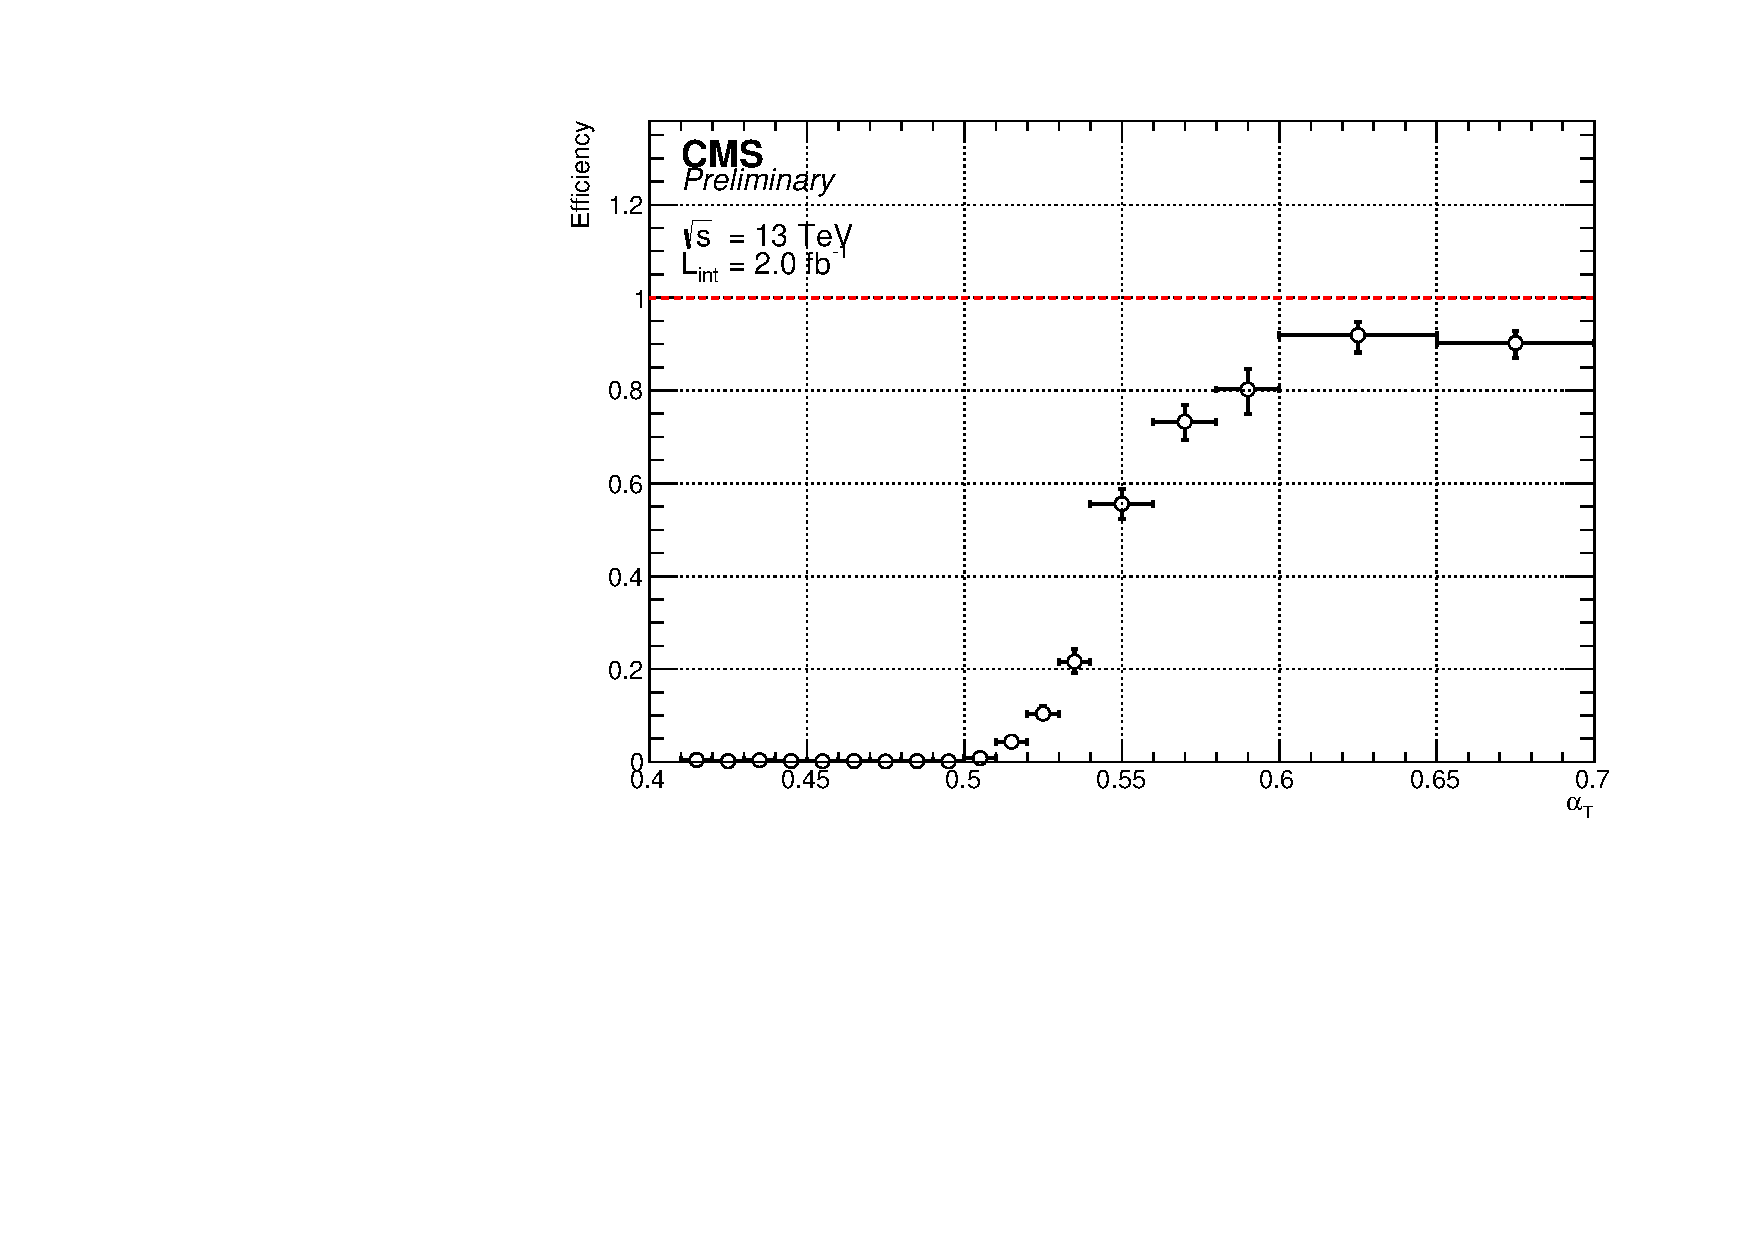
\includegraphics[width=0.5\textwidth]{figures/Trigger/HLT_Ele23_eta2p1_WPLoose_Gsf/HLT_PFHT200_DiPFJetAve90_PFAlphaT0p57_MoM_HT300_alphaT}} ~~
    \subfigure[{\tiny HLT\_PFHT200\_DiPFJetAve90\_PFAlphaT0p57 ($\alt>0.60$)}]{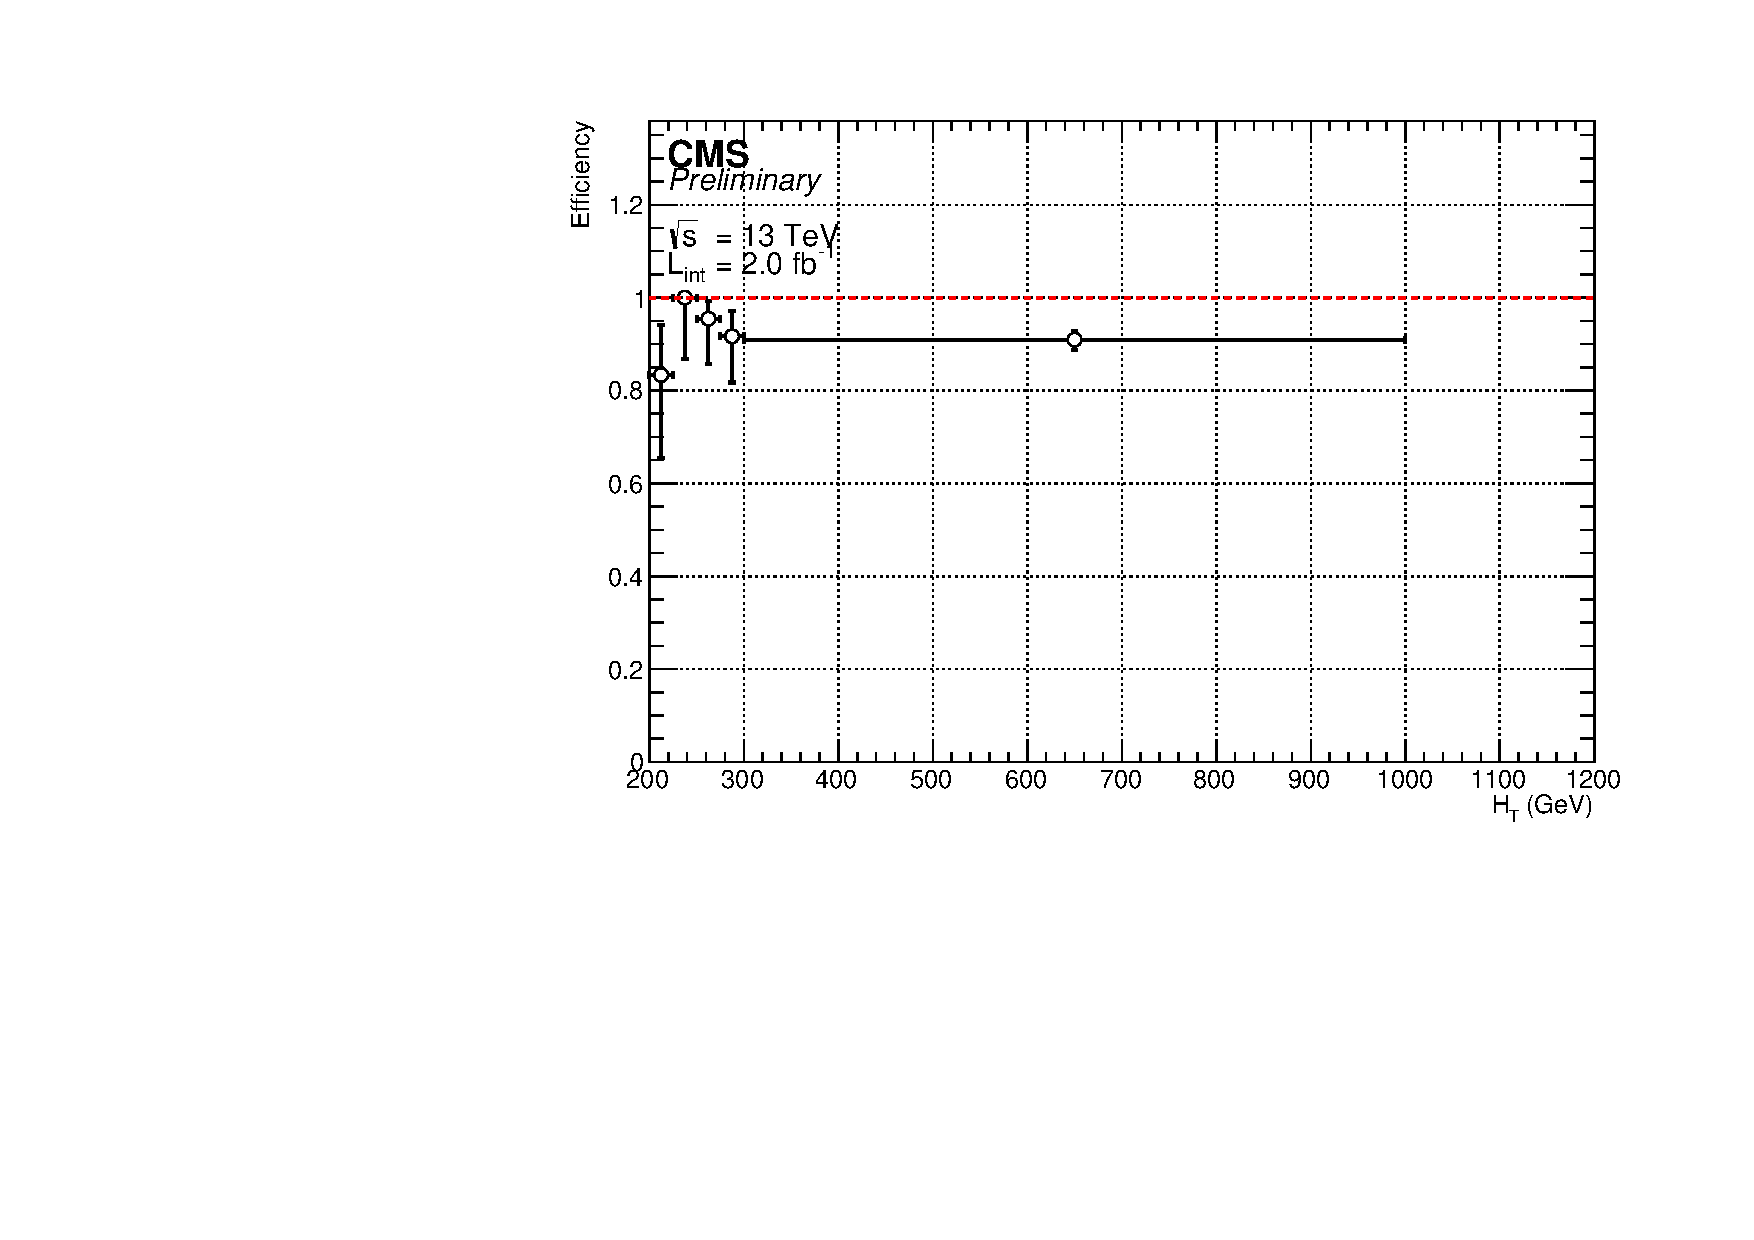
\includegraphics[width=0.5\textwidth]{figures/Trigger/HLT_Ele23_eta2p1_WPLoose_Gsf/HLT_PFHT200_DiPFJetAve90_PFAlphaT0p57_MoM_aT0p60_ht}} \\
    \subfigure[{\tiny HLT\_PFHT300\_DiPFJetAve90\_PFAlphaT0p53 ($\scalht>400$~GeV)}]{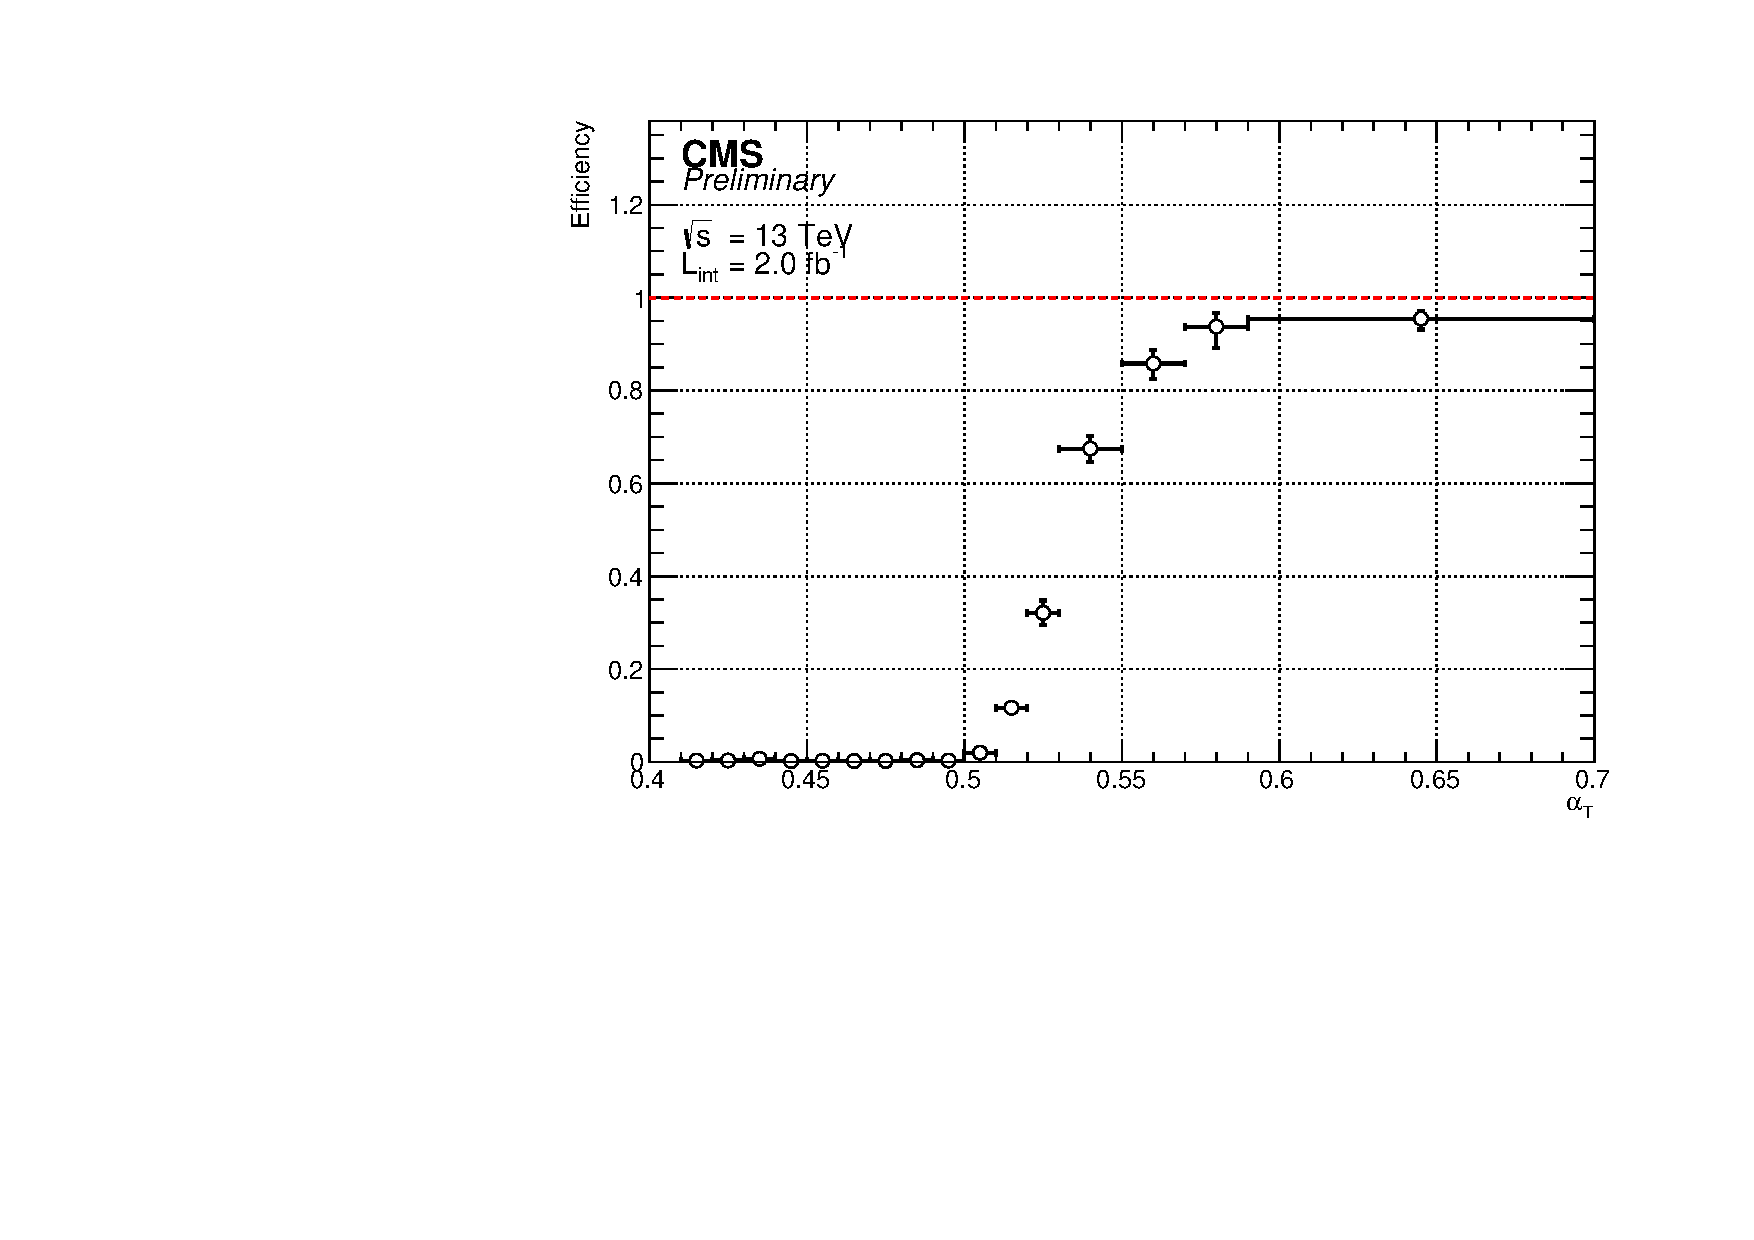
\includegraphics[width=0.5\textwidth]{figures/Trigger/HLT_Ele23_eta2p1_WPLoose_Gsf/HLT_PFHT300_DiPFJetAve90_PFAlphaT0p53_MoM_HT400_alphaT}} ~~
    \subfigure[{\tiny HLT\_PFHT300\_DiPFJetAve90\_PFAlphaT0p53 ($\alt>0.58$)}]{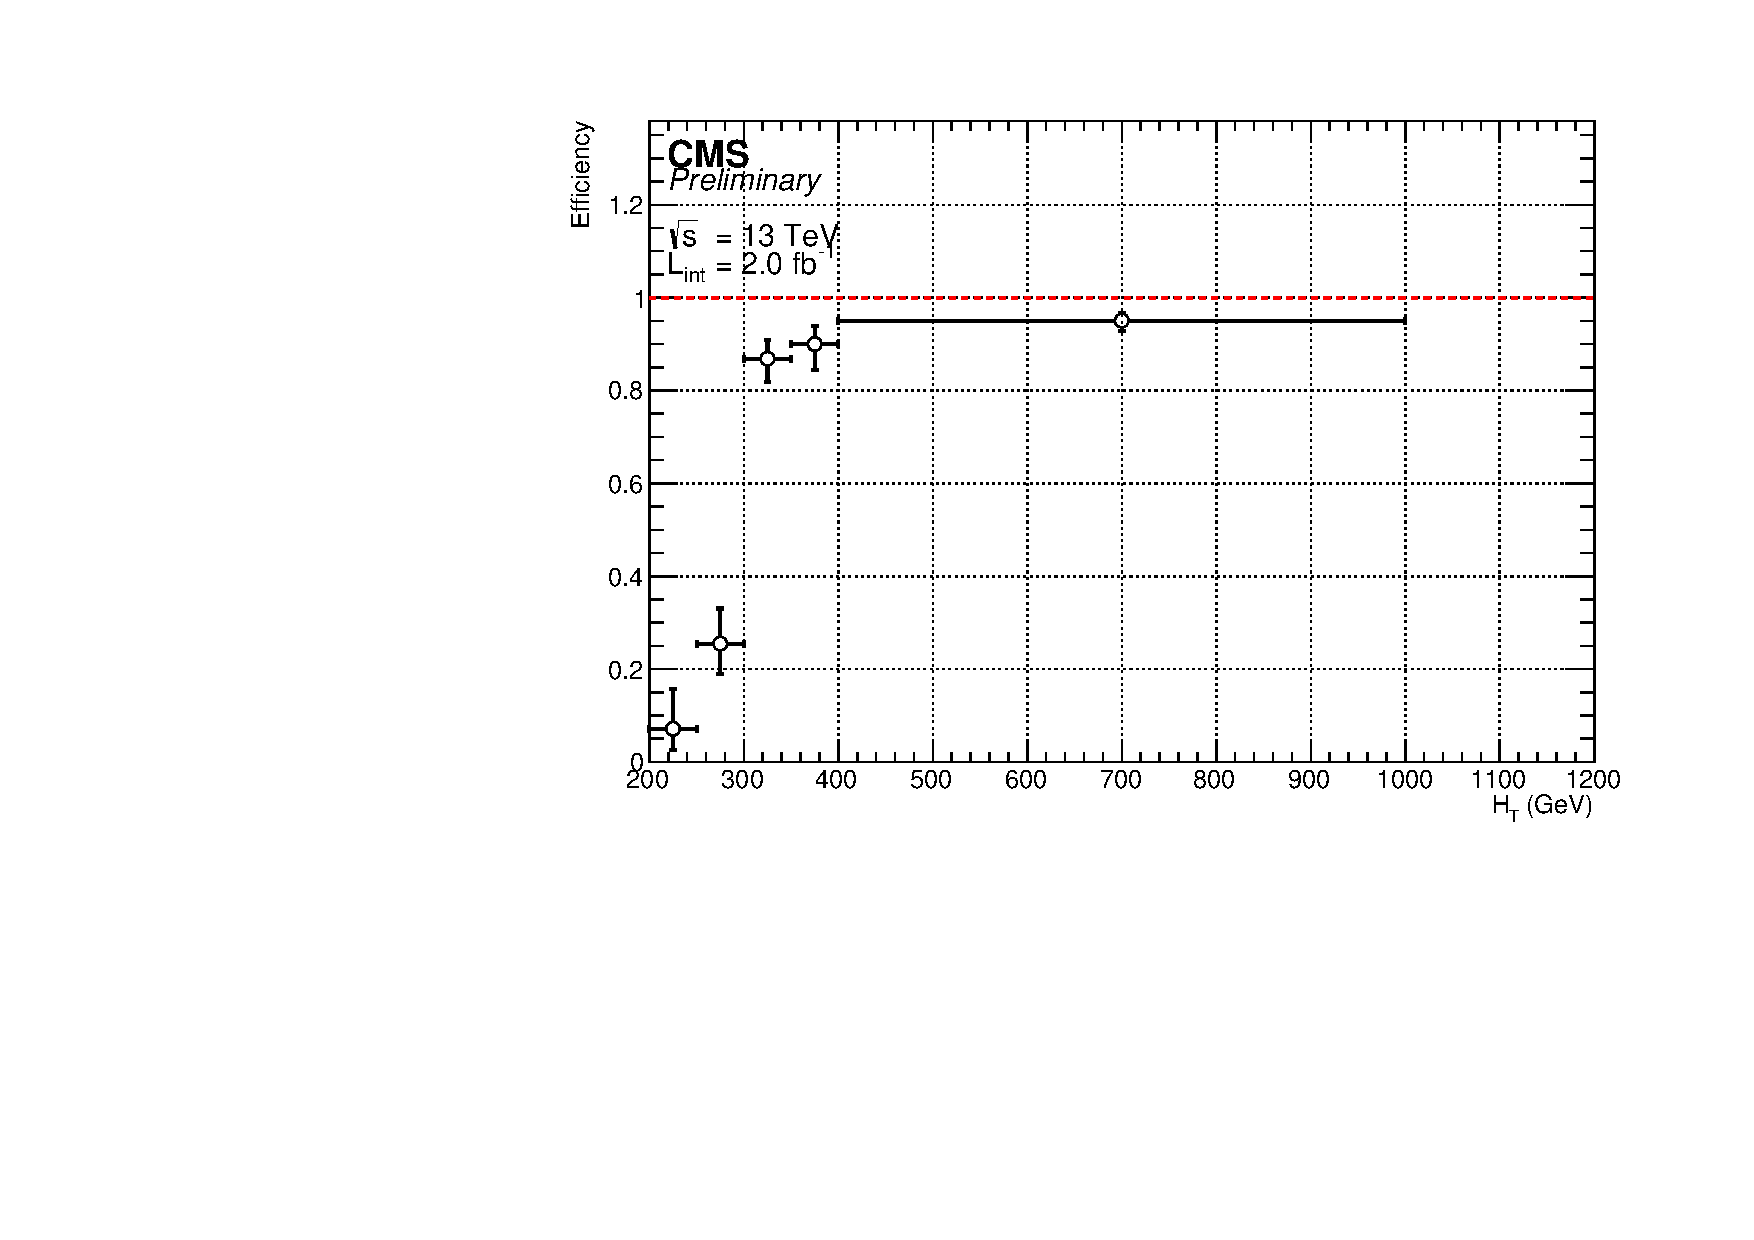
\includegraphics[width=0.5\textwidth]{figures/Trigger/HLT_Ele23_eta2p1_WPLoose_Gsf/HLT_PFHT300_DiPFJetAve90_PFAlphaT0p53_MoM_aT0p58_ht}} \\
    \subfigure[{\tiny HLT\_PFHT400\_DiPFJetAve90\_PFAlphaT0p51 ($\scalht>500$~GeV)}]{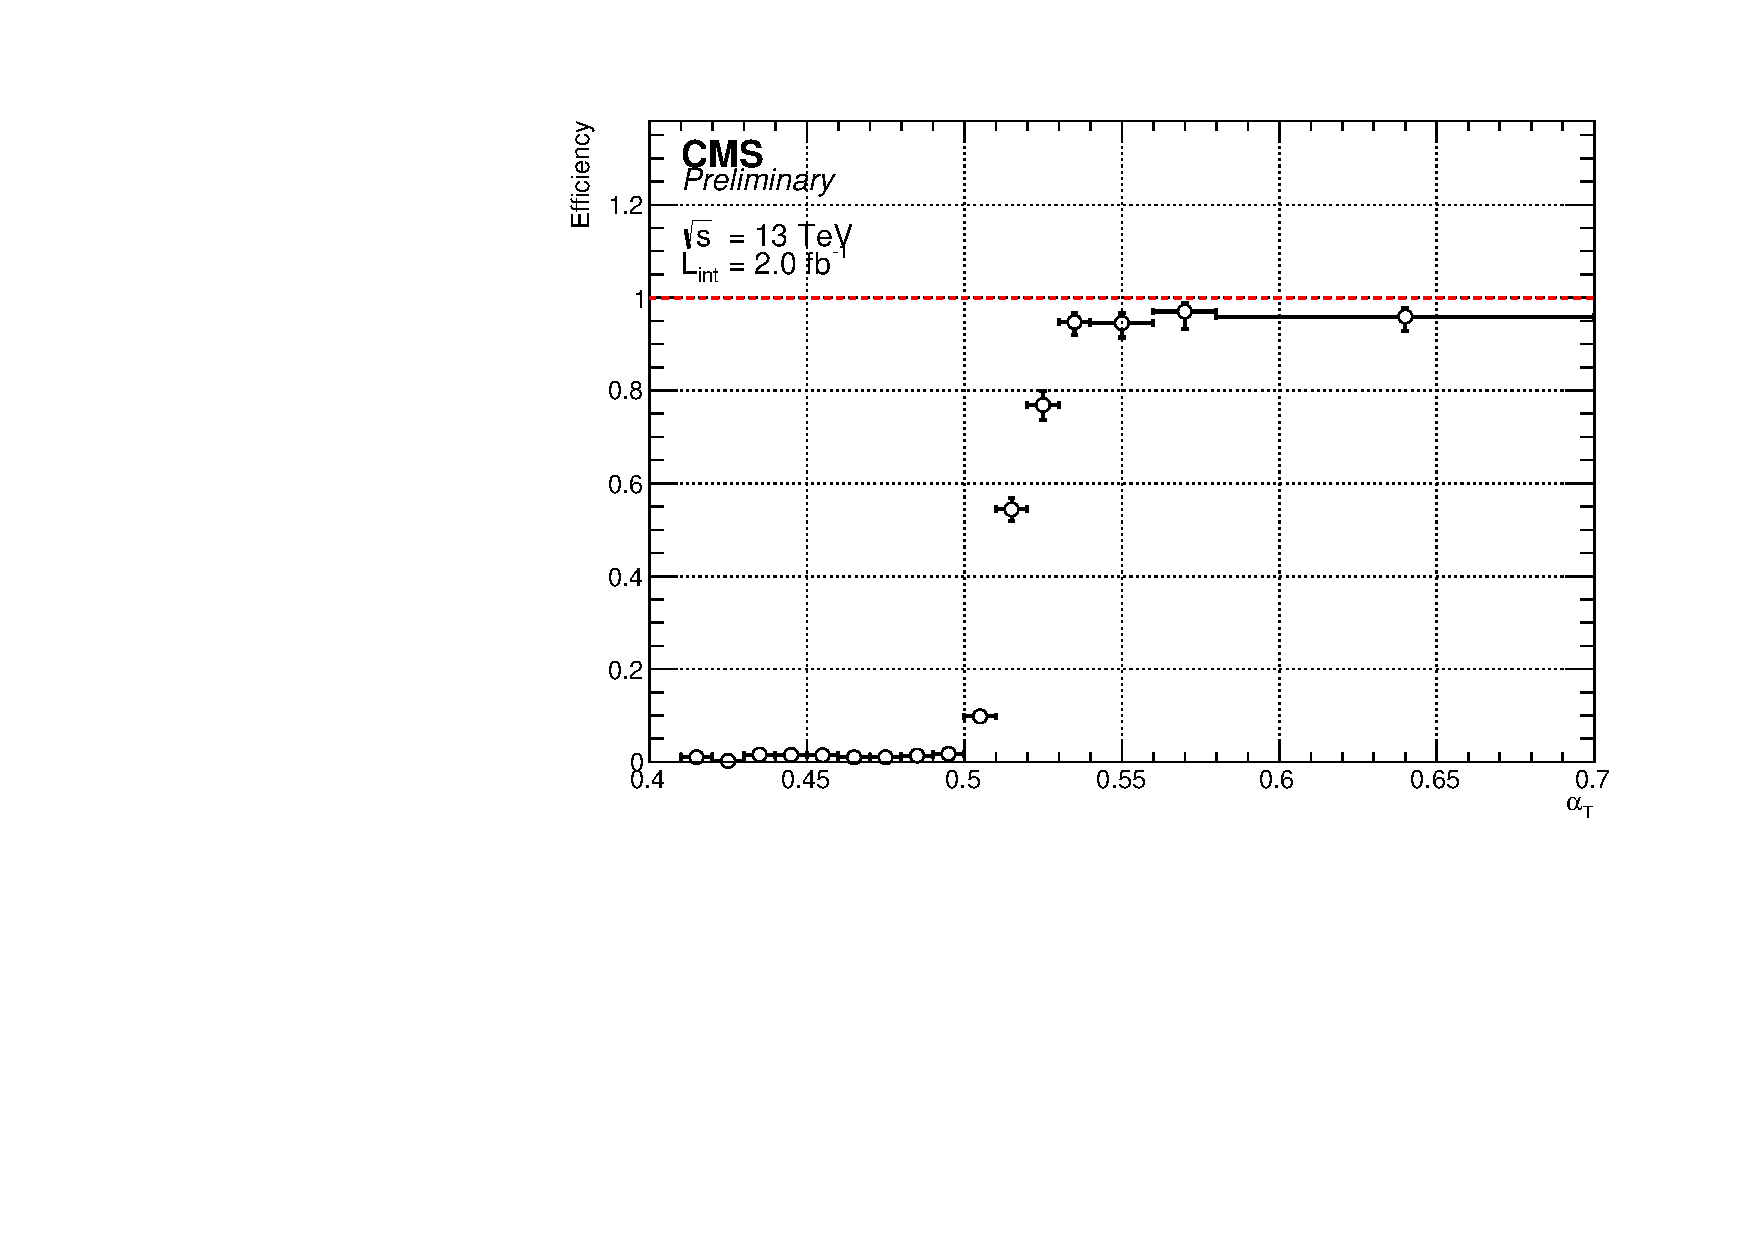
\includegraphics[width=0.5\textwidth]{figures/Trigger/HLT_Ele23_eta2p1_WPLoose_Gsf/HLT_PFHT400_DiPFJetAve90_PFAlphaT0p51_MoM_HT500_alphaT}} ~~
    \subfigure[{\tiny HLT\_PFHT400\_DiPFJetAve90\_PFAlphaT0p51 ($\alt>0.55$)}]{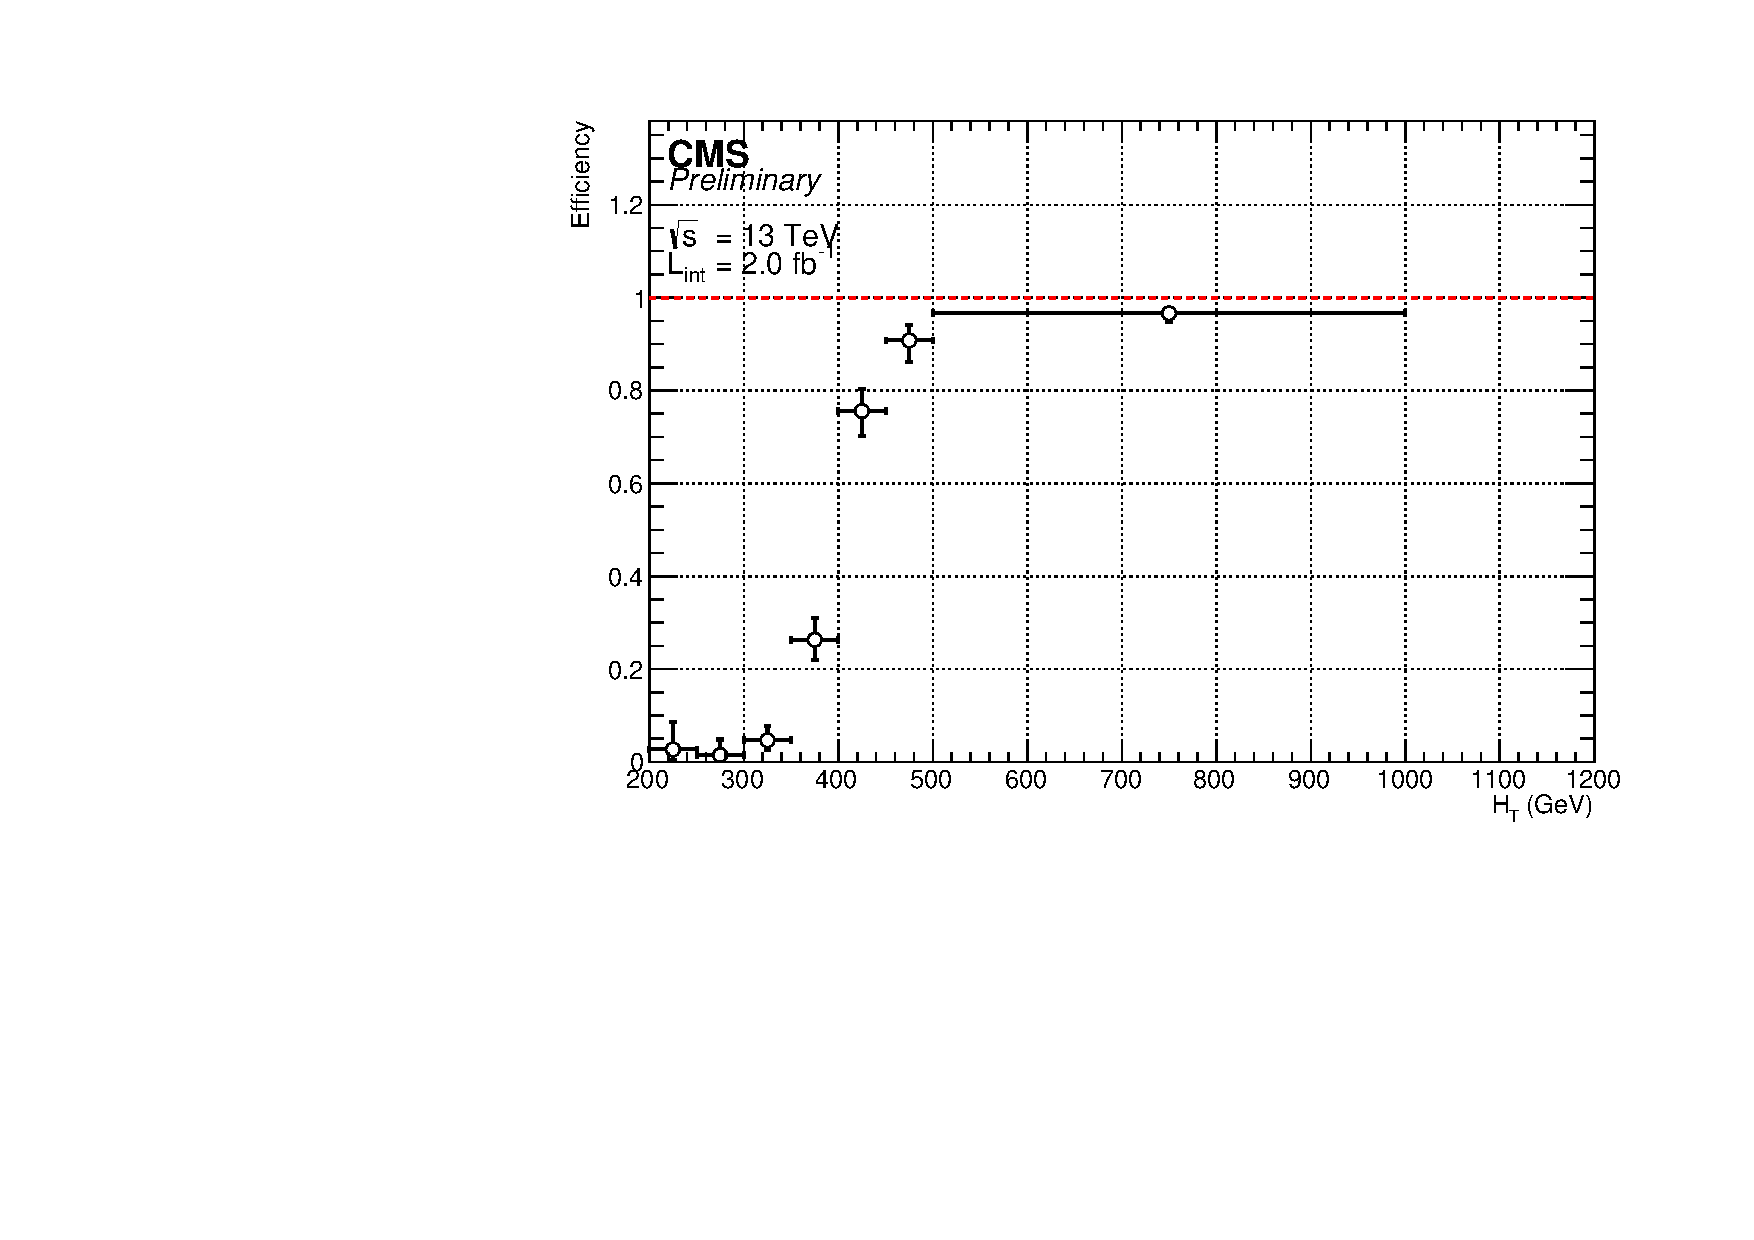
\includegraphics[width=0.5\textwidth]{figures/Trigger/HLT_Ele23_eta2p1_WPLoose_Gsf/HLT_PFHT400_DiPFJetAve90_PFAlphaT0p51_MoM_aT0p55_ht}} ~~
    \caption{
      The trigger efficiency measured in the data as a function of \alt and \scalht in the symmetric categories for the \scalht-\alt triggers used to seed the analysis bins in the signal region. The offline \alt or \scalht cuts applied to ensure full efficiency in the opposite leg are also specified. 
    }
    \label{fig:alphat_turnons}
  \end{center} 
\end{figure}

\newpage
Figure \ref{fig:turnons_njetbinned} shows \mht turn-ons in the low \scalht signal region in bins of \njet. 
No significant dependence is observed, and no unexpected inefficiencies are evident at high \njet, 
low \scalht.

\begin{figure}[h!]
  \begin{center}

    \subfigure[{\tiny $\scalht = 200\mathrm-250$~GeV, $\njet = 1$}]{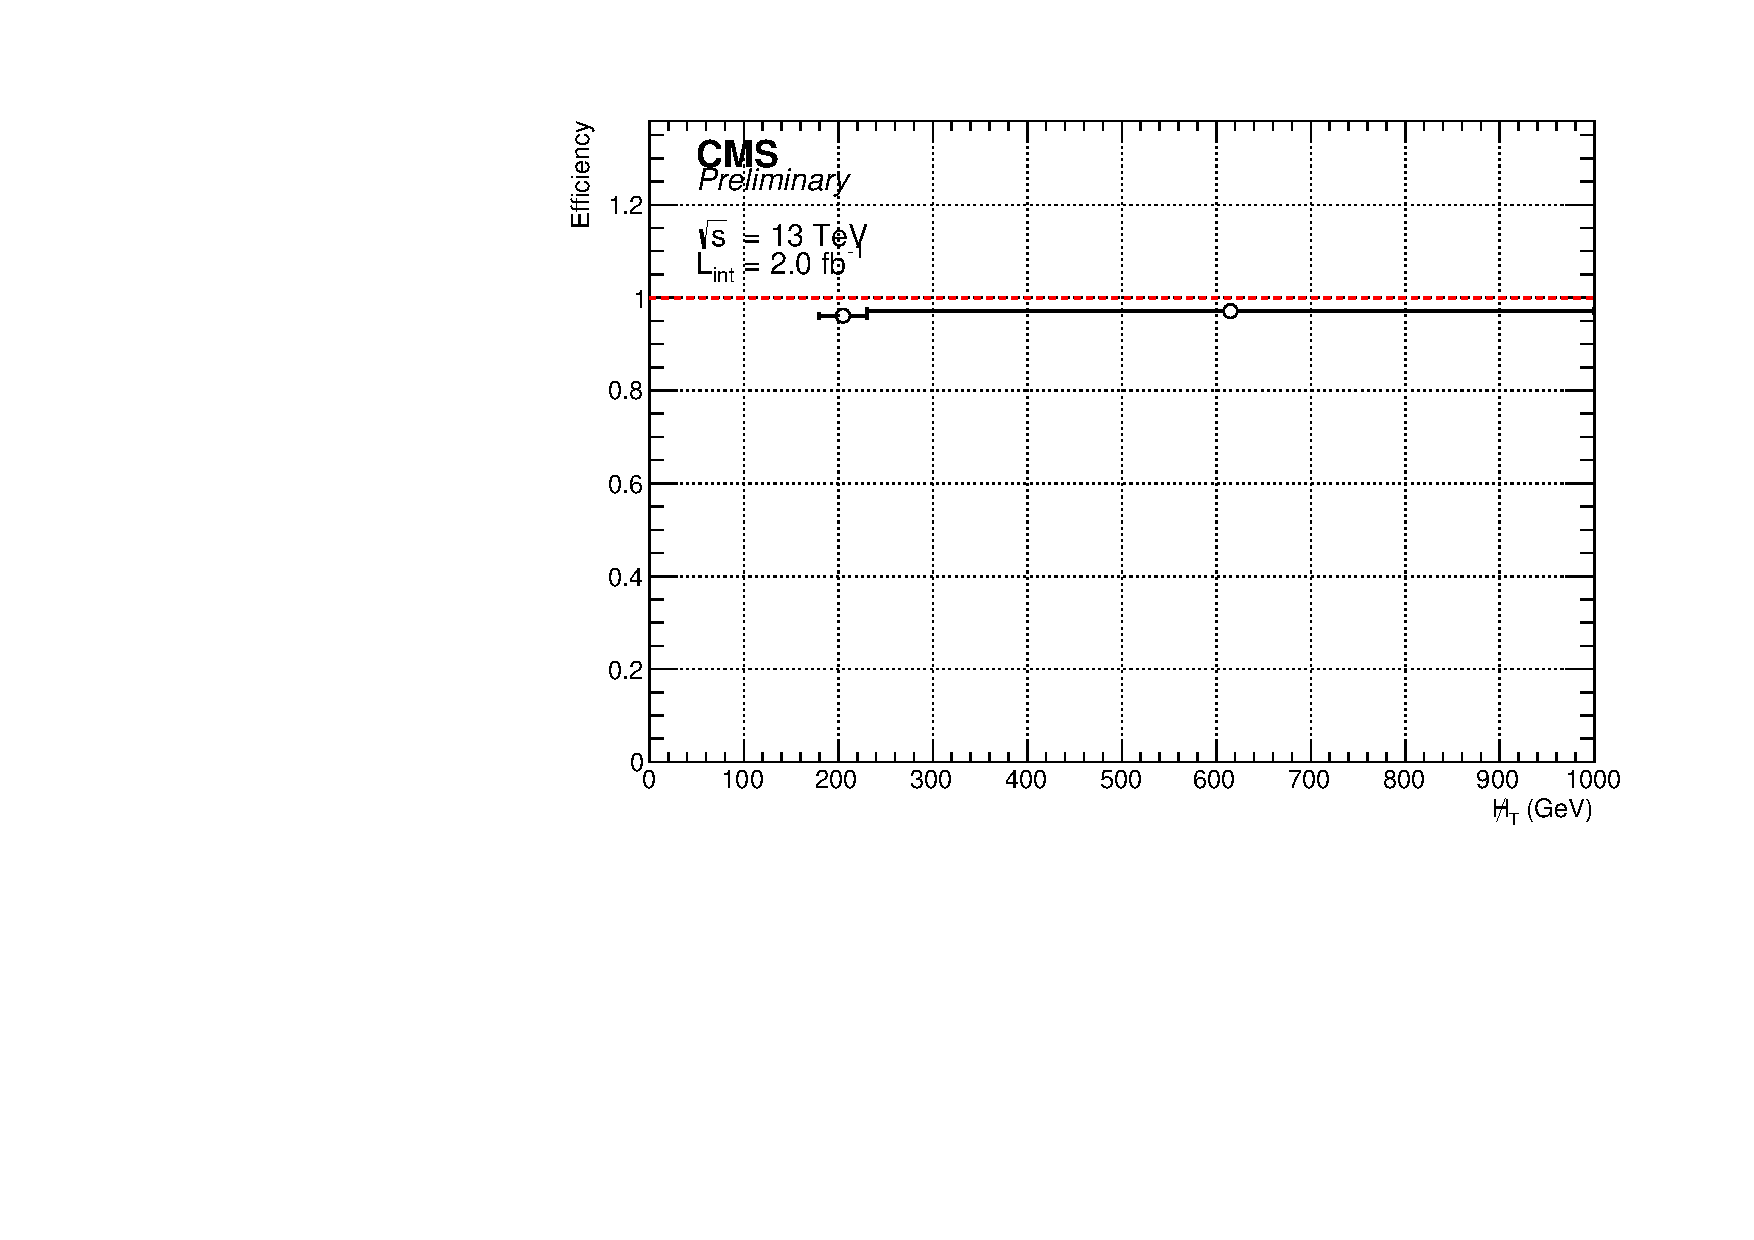
\includegraphics[width=0.4\textwidth]{figures/Trigger/NJetBinned/HLT_AlphaTMonoAll_MoM_eq1j_200to250_mht}} \\
    \subfigure[{\tiny $\scalht = 200\mathrm-250$~GeV, $\njet = 2$ sym.}]{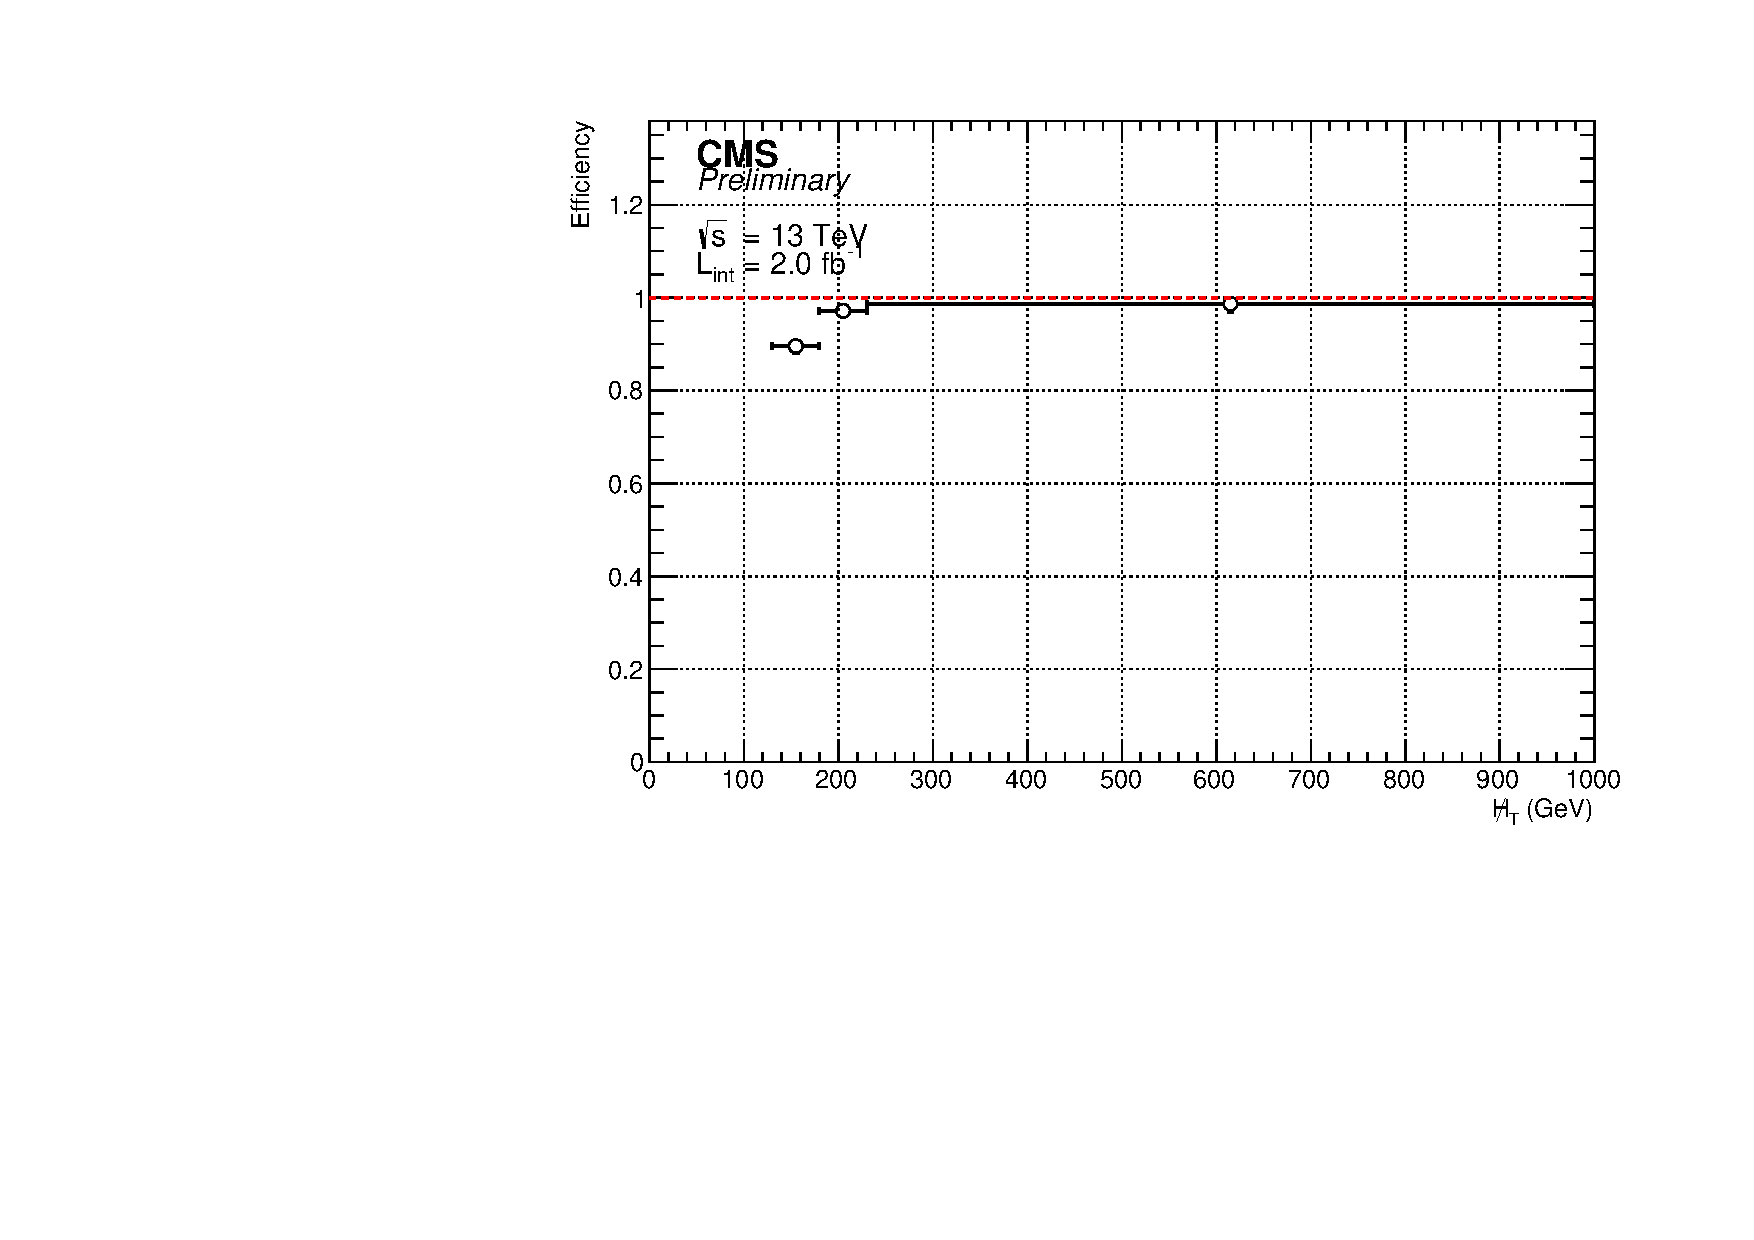
\includegraphics[width=0.4\textwidth]{figures/Trigger/NJetBinned/HLT_AlphaTMonoAll_MoM_eq2j_200to250_mht}} 
    \subfigure[{\tiny $\scalht = 200\mathrm-250$~GeV, $\njet = 3$ sym.}]{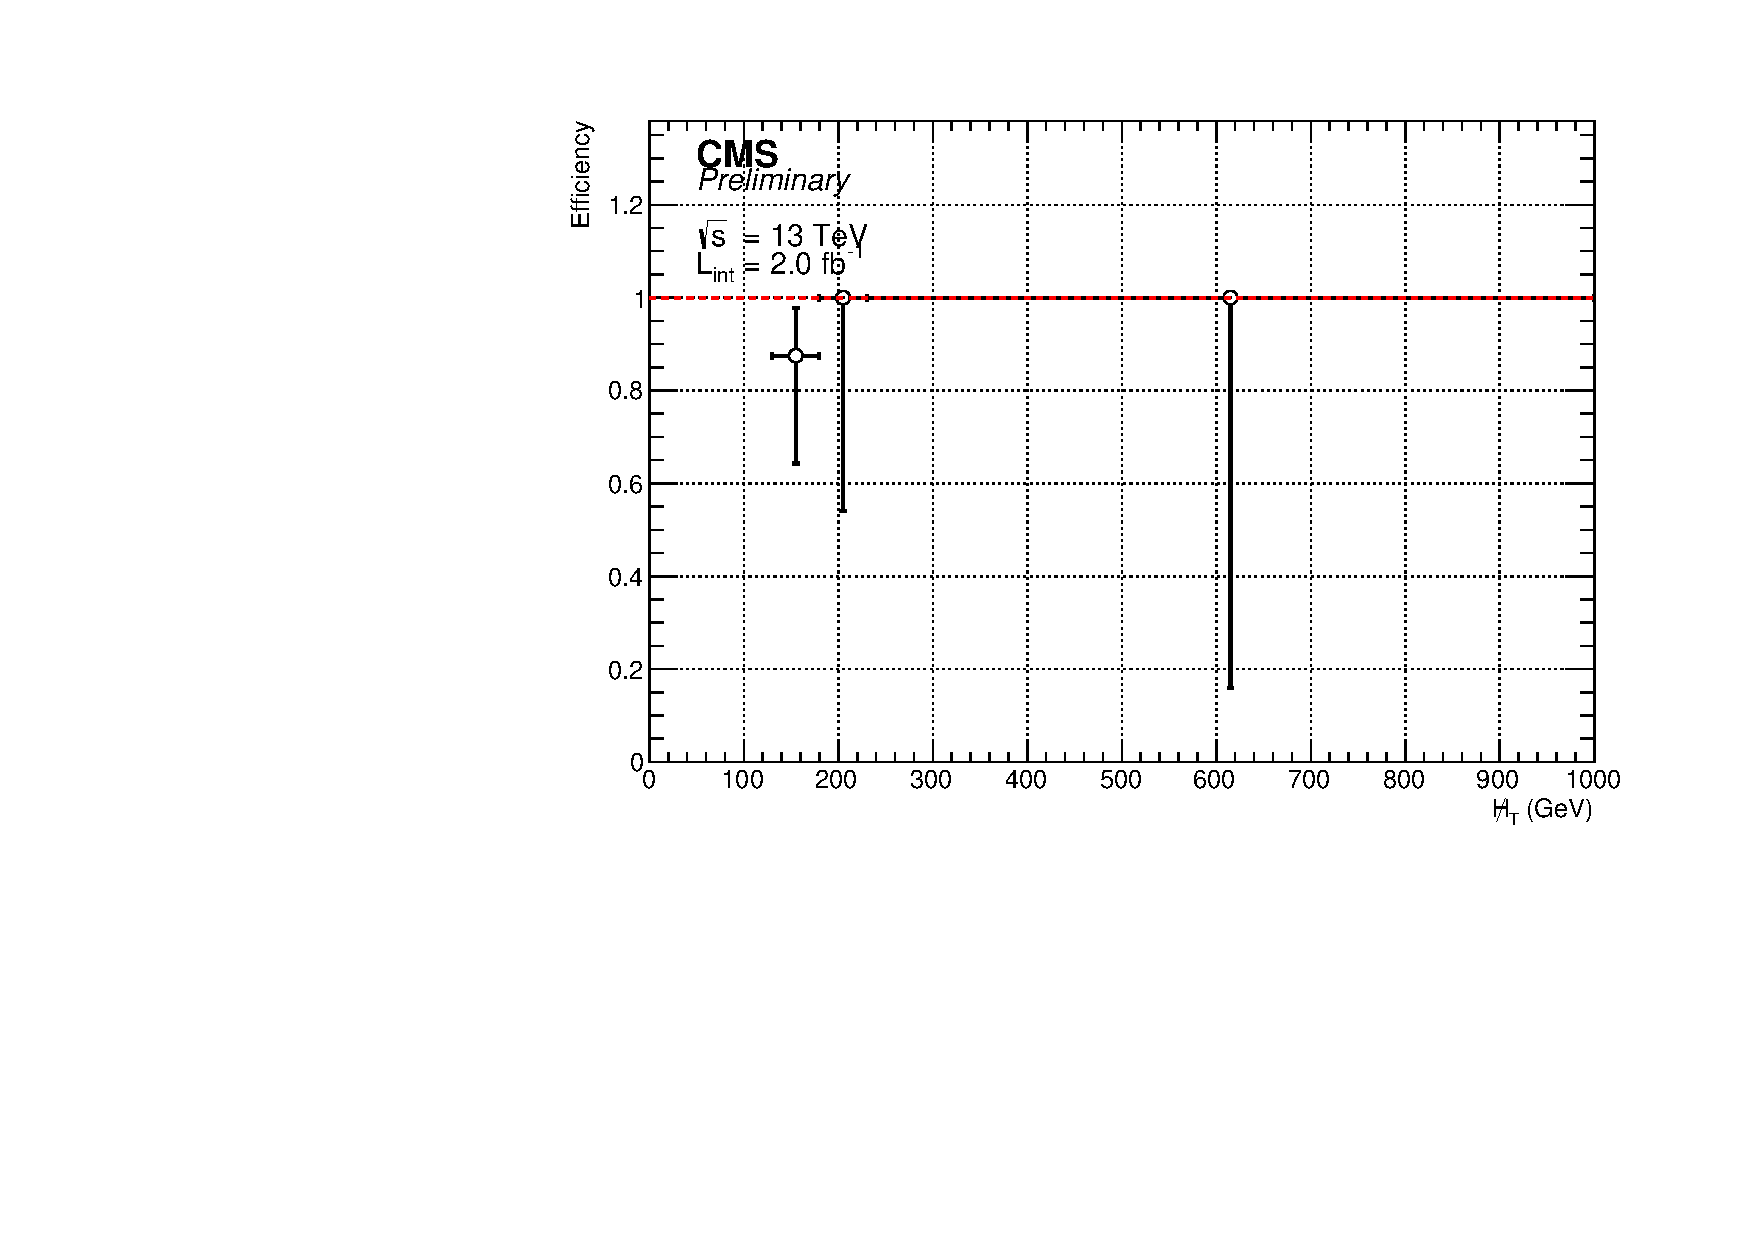
\includegraphics[width=0.4\textwidth]{figures/Trigger/NJetBinned/HLT_AlphaTMonoAll_MoM_eq3j_200to250_mht}} \\
    \subfigure[{\tiny $\scalht = 200\mathrm-250$~GeV, $\njet = 2$ asym.}]{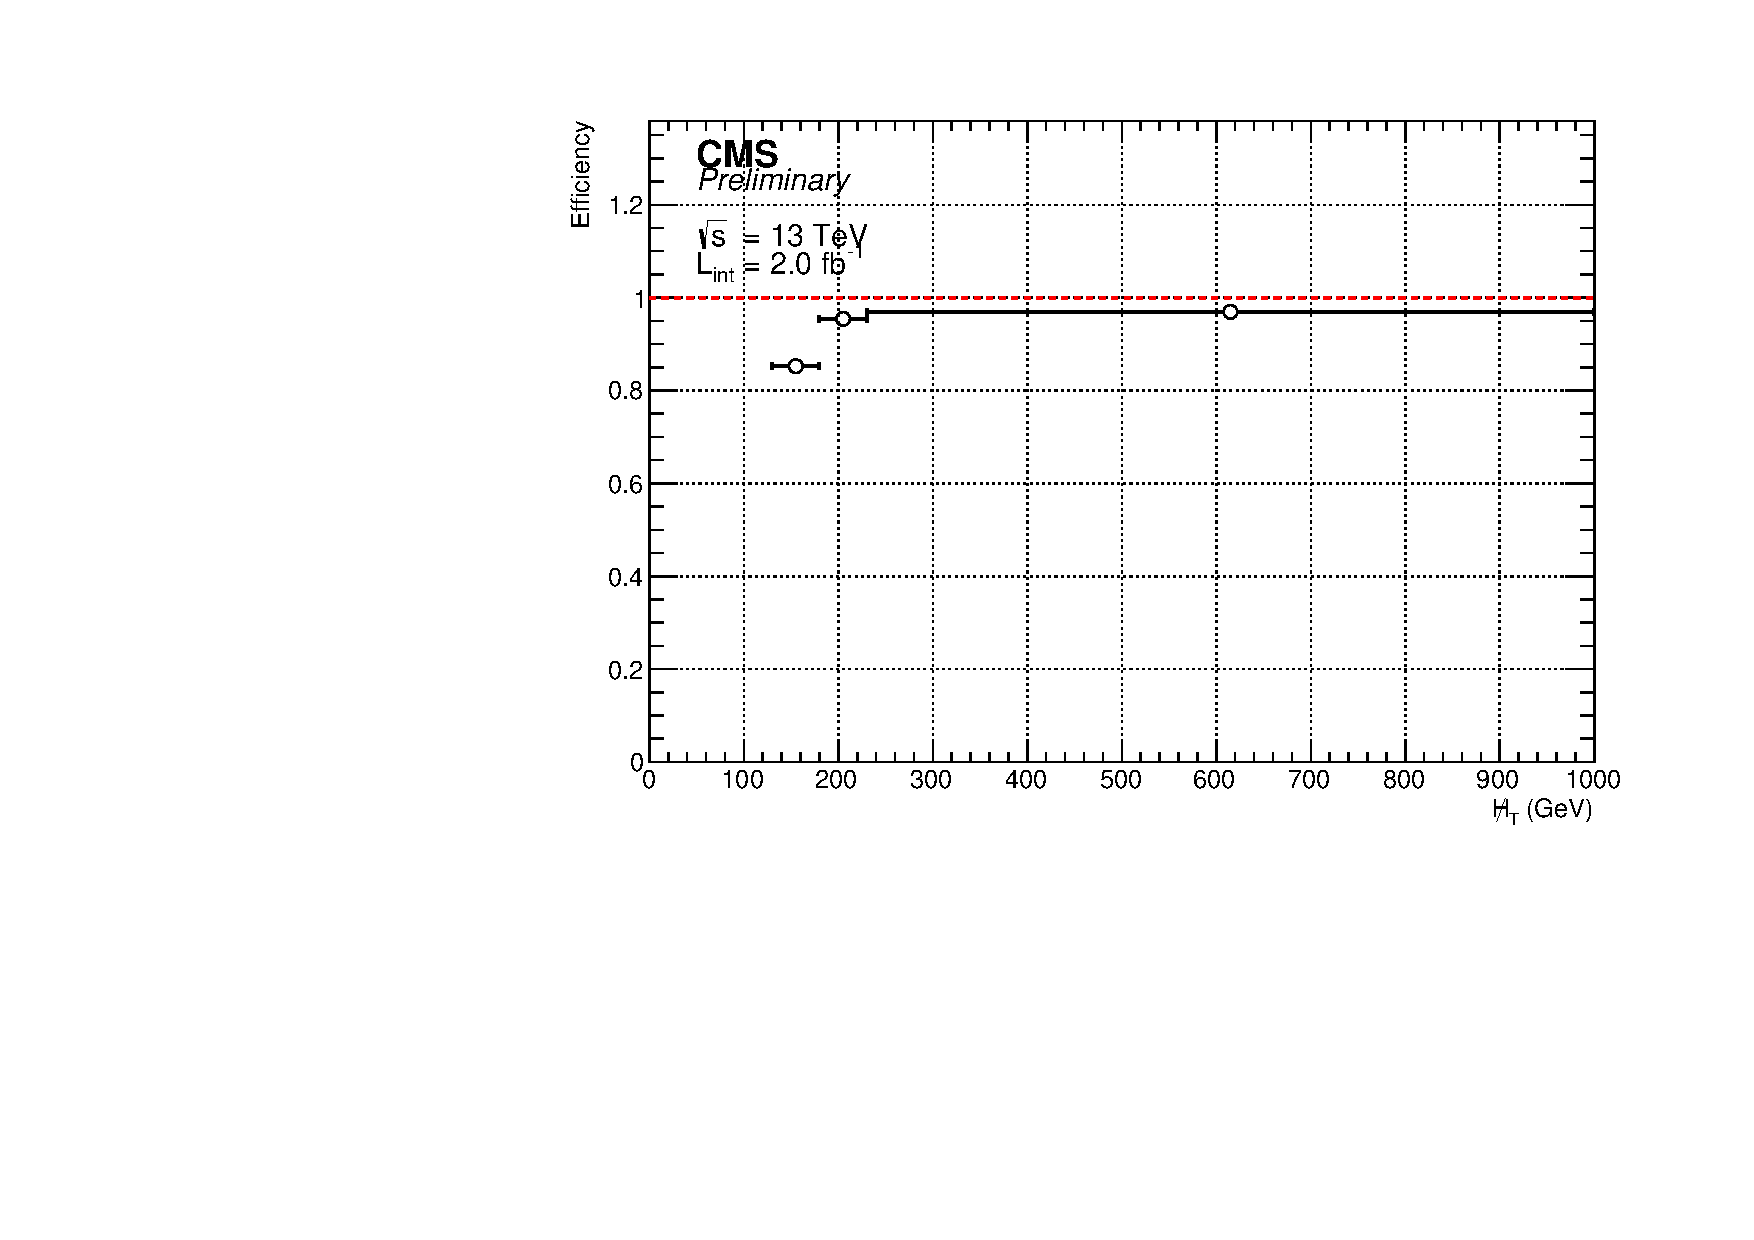
\includegraphics[width=0.4\textwidth]{figures/Trigger/NJetBinned/HLT_AlphaTMonoAll_MoM_eq2a_200to250_mht}}
    \subfigure[{\tiny $\scalht = 200\mathrm-250$~GeV, $\njet = 3$ asym.}]{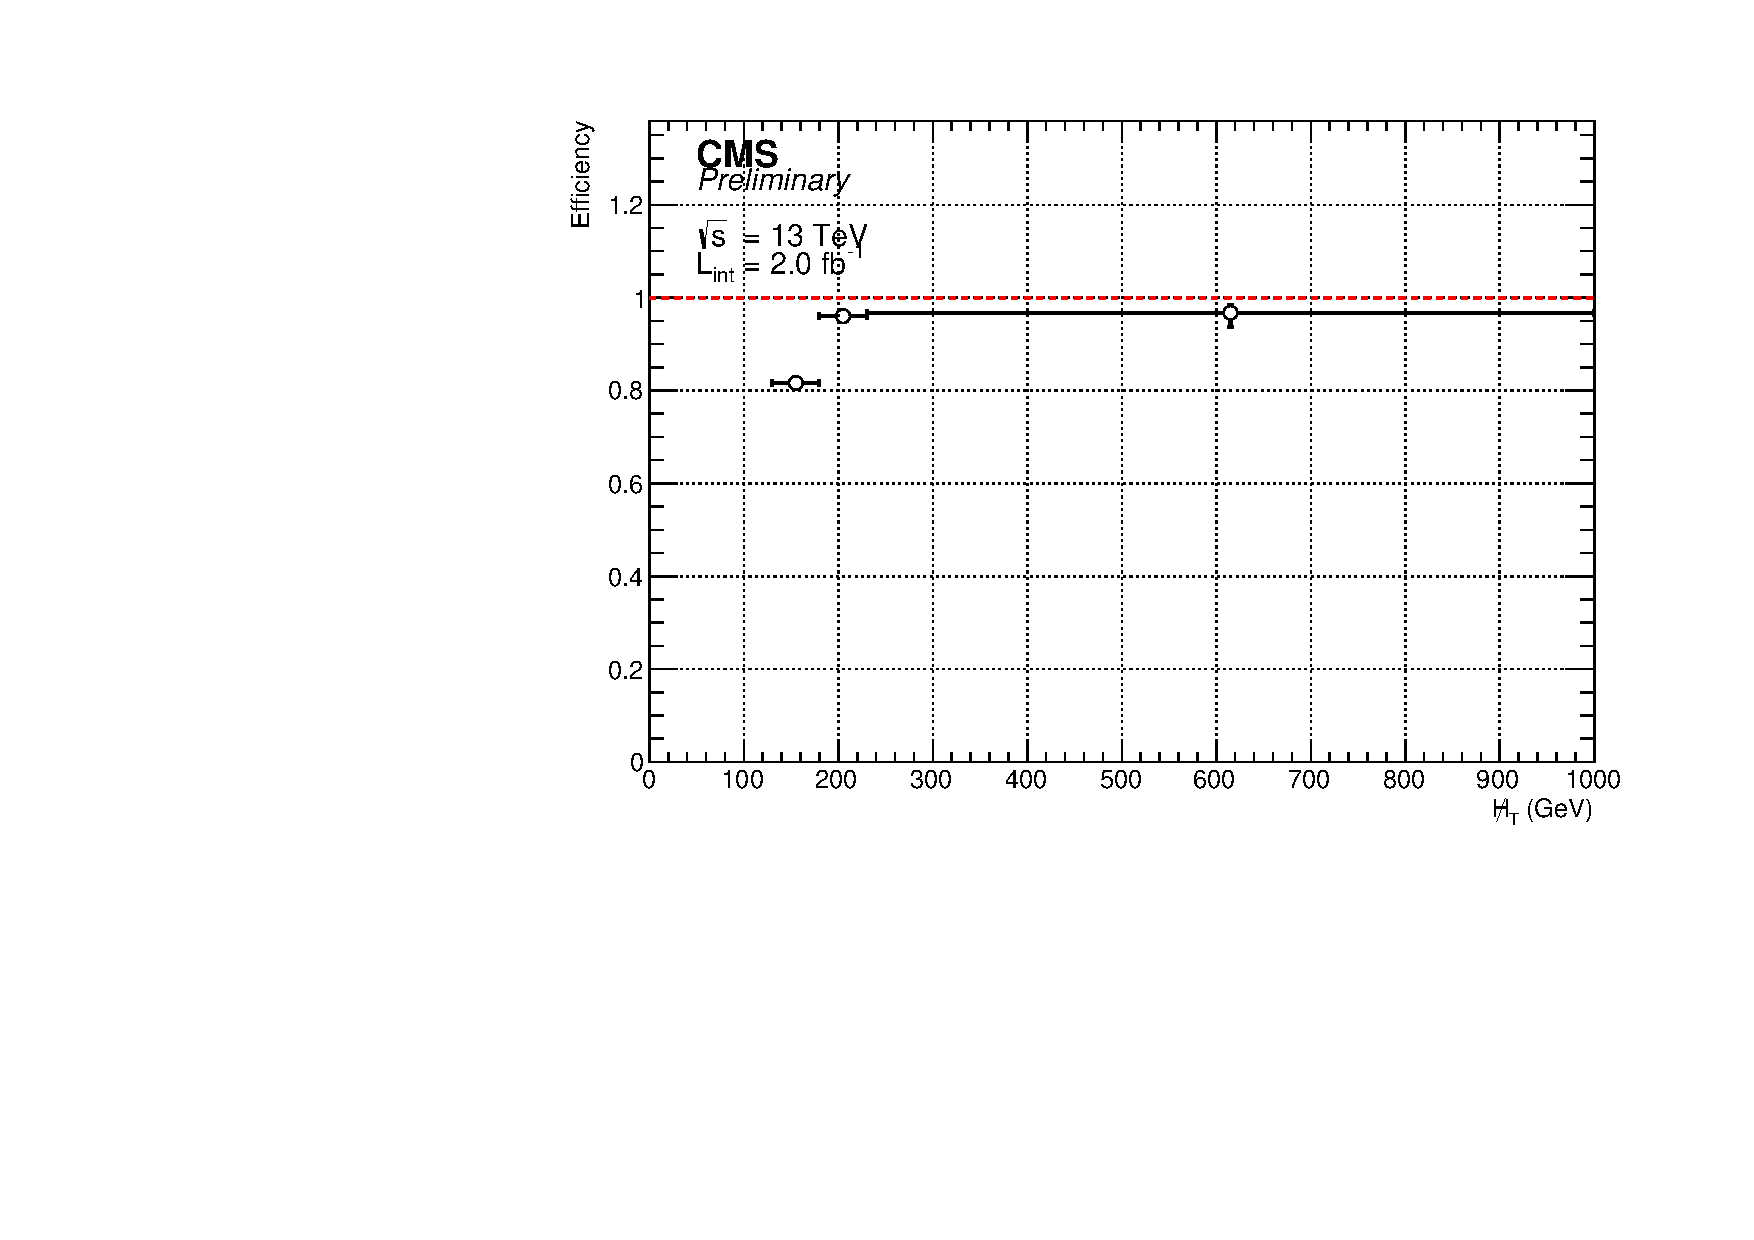
\includegraphics[width=0.4\textwidth]{figures/Trigger/NJetBinned/HLT_AlphaTMonoAll_MoM_eq3a_200to250_mht}} \\ 
  \end{center}
\end{figure}
\newpage
\begin{figure}[h!]
  \begin{center}    
    \subfigure[{\tiny $\scalht = 250\mathrm-300$~GeV, $\njet = 1$}]{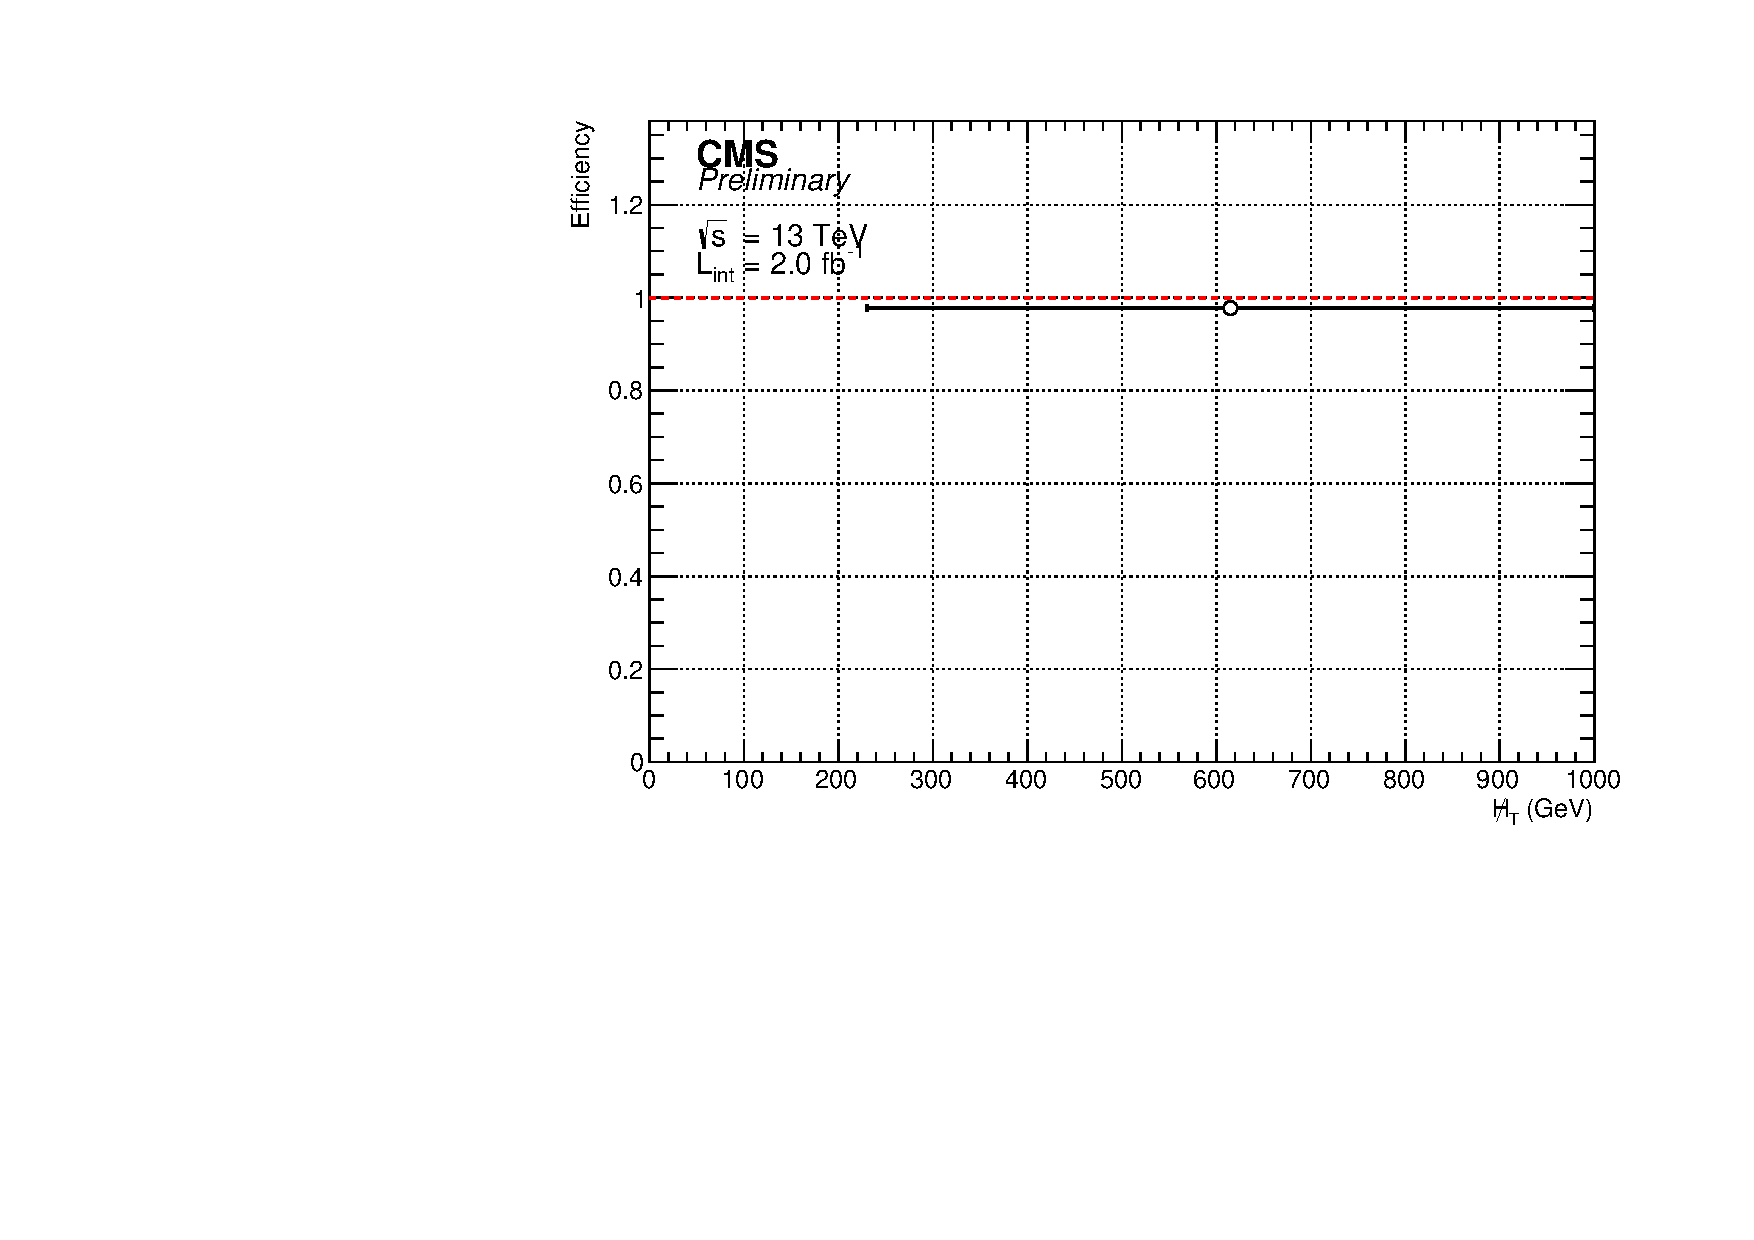
\includegraphics[width=0.4\textwidth]{figures/Trigger/NJetBinned/HLT_AlphaTMonoAll_MoM_eq1j_250to300_mht}}
    \subfigure[{\tiny $\scalht = 250\mathrm-300$~GeV, $\njet = 2$ sym.}]{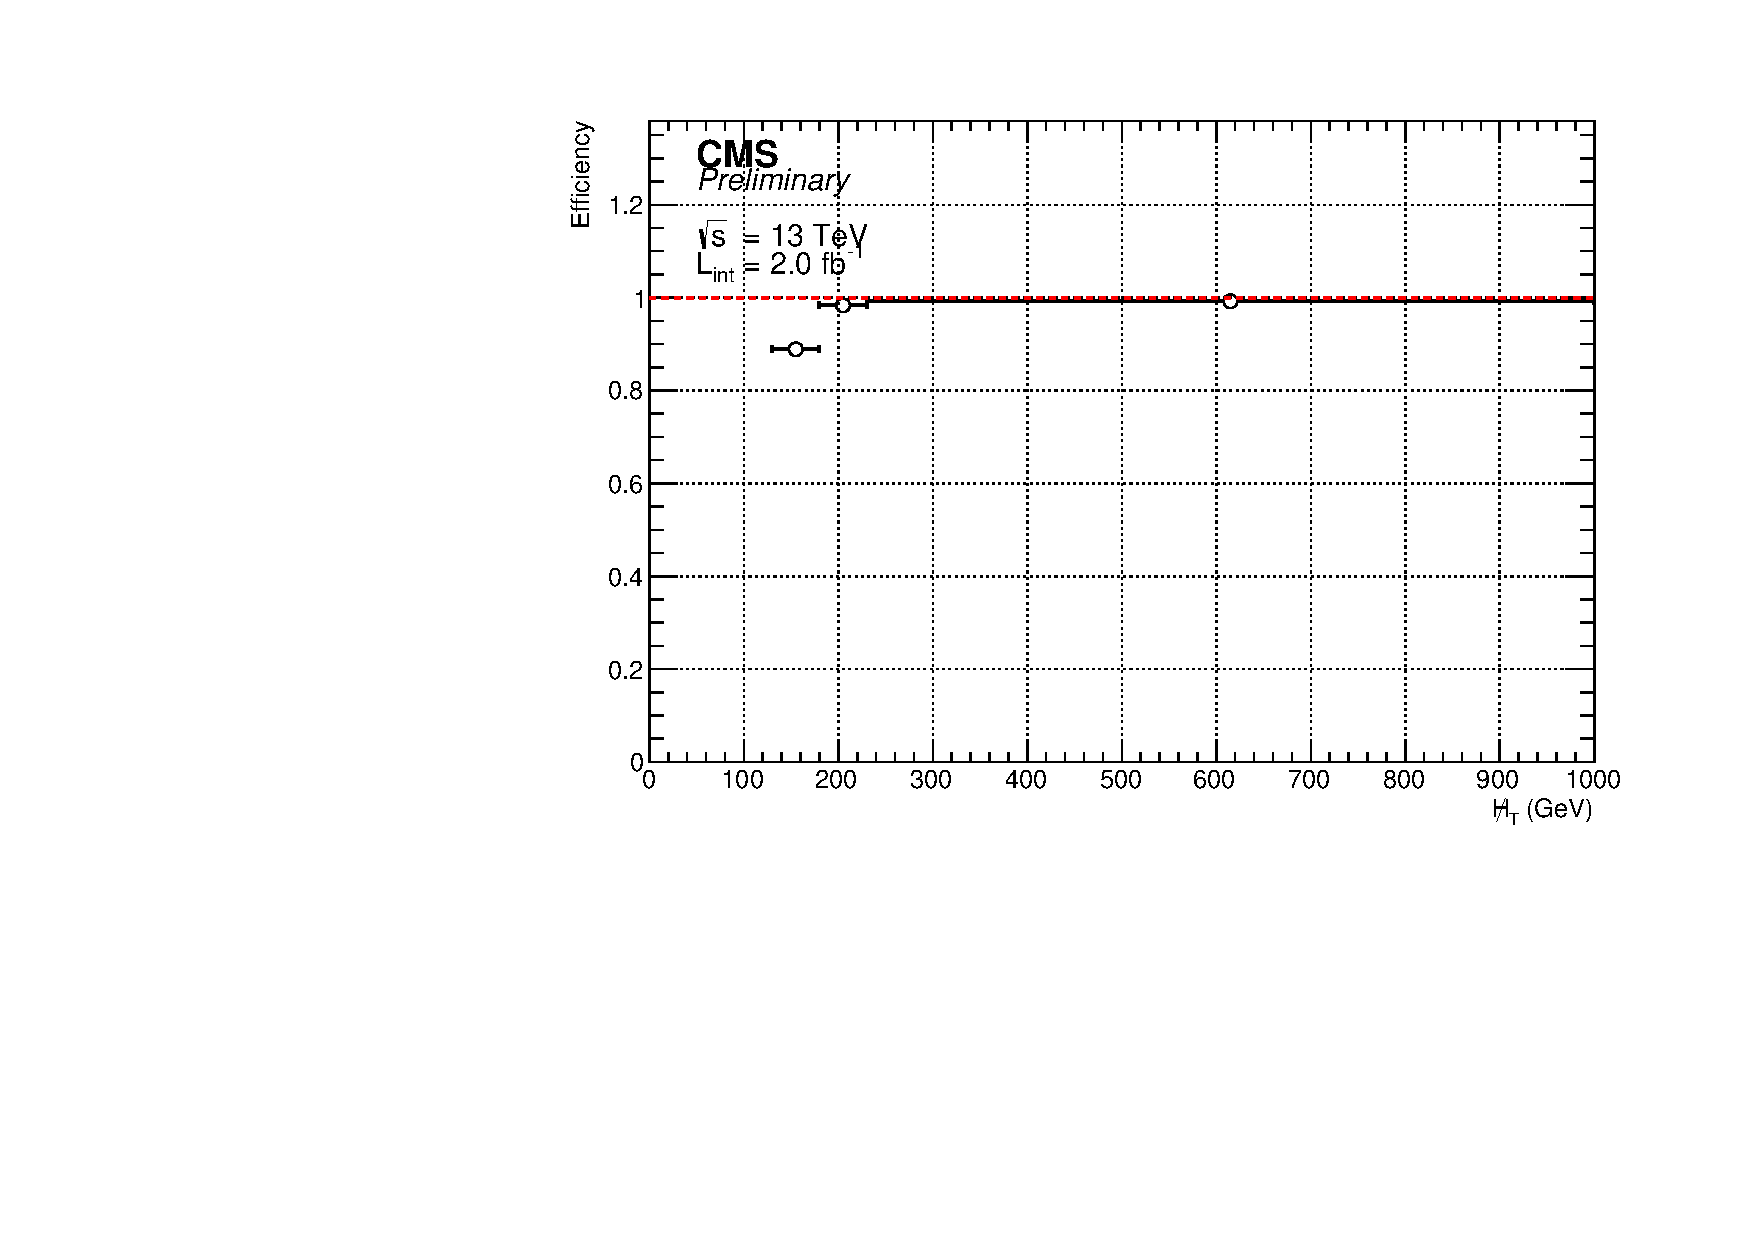
\includegraphics[width=0.4\textwidth]{figures/Trigger/NJetBinned/HLT_AlphaTMonoAll_MoM_eq2j_250to300_mht}} \\
    \subfigure[{\tiny $\scalht = 250\mathrm-300$~GeV, $\njet = 3$ sym.}]{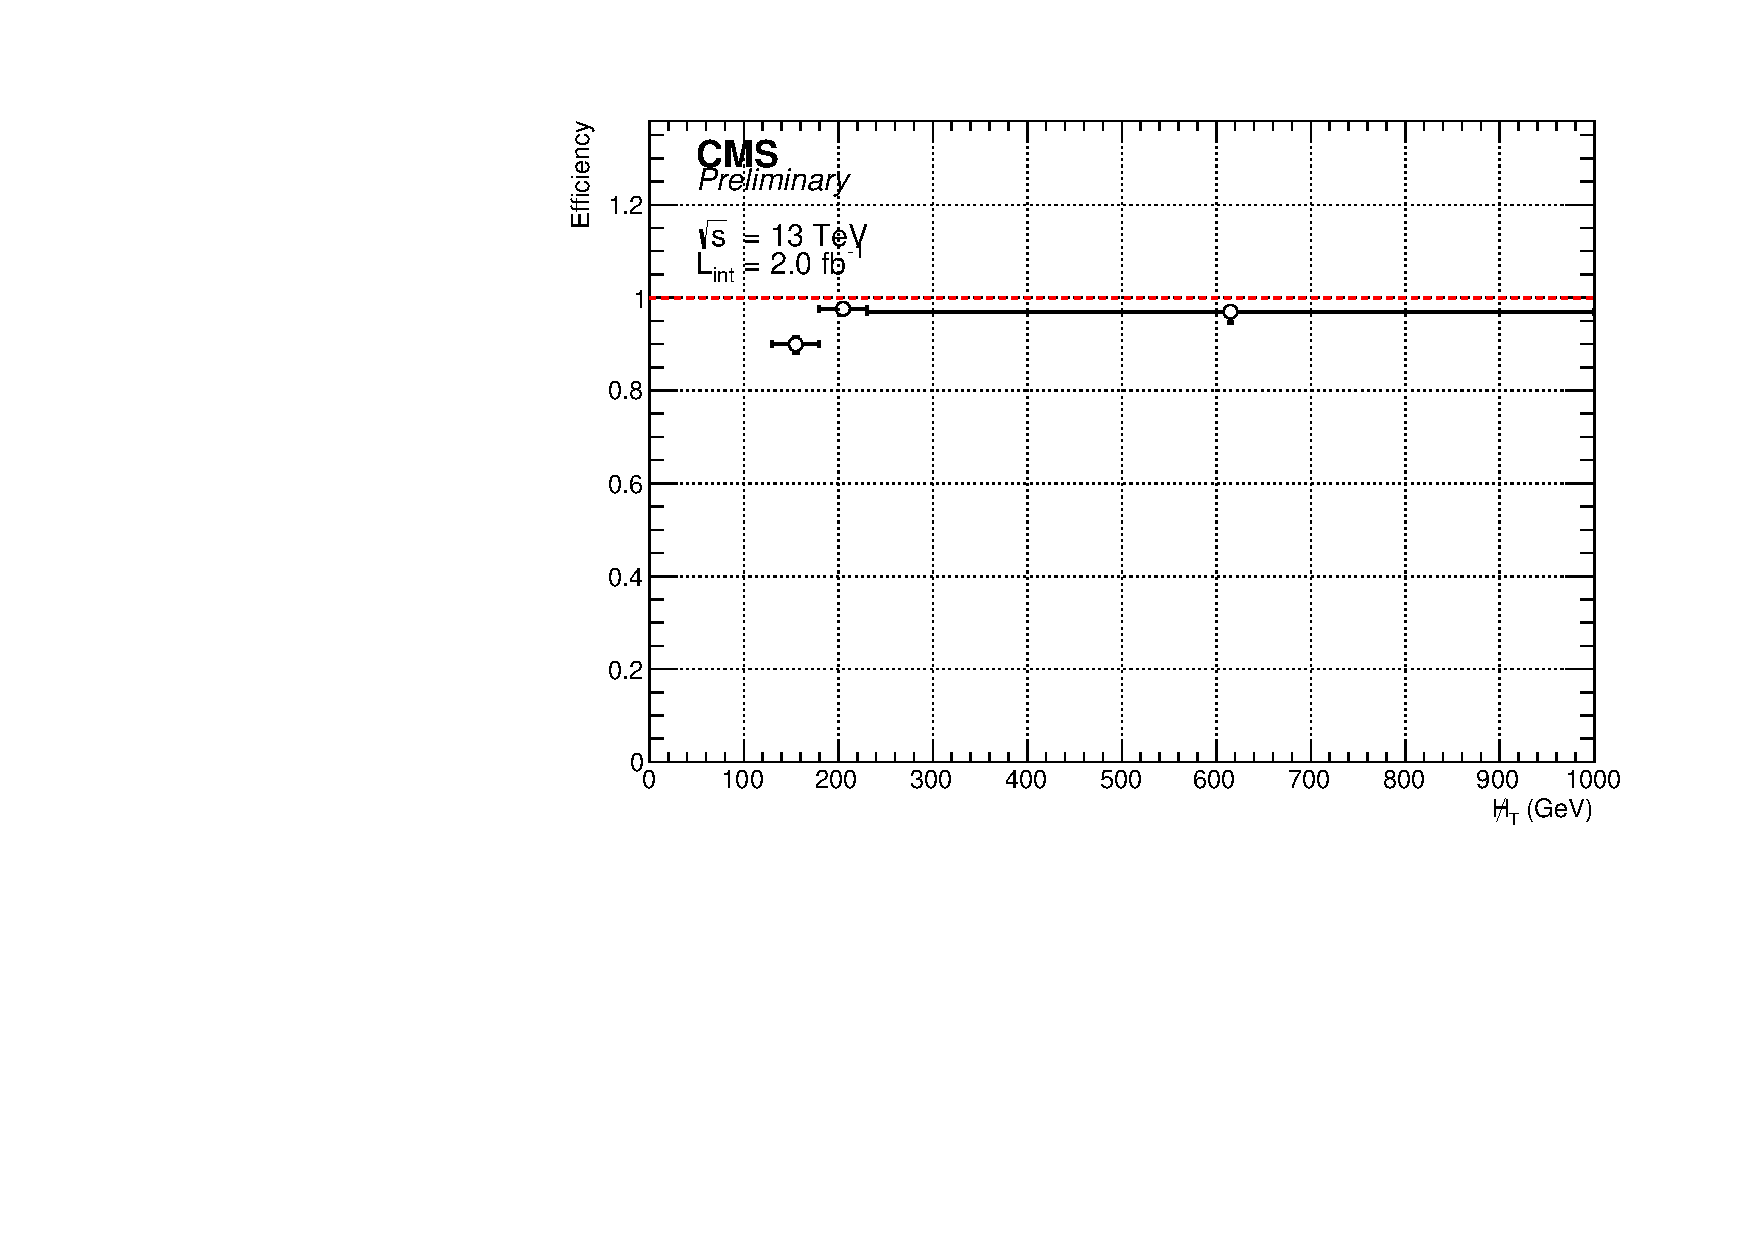
\includegraphics[width=0.4\textwidth]{figures/Trigger/NJetBinned/HLT_AlphaTMonoAll_MoM_eq3j_250to300_mht}}
    \subfigure[{\tiny $\scalht = 250\mathrm-300$~GeV, $\njet = 4$ sym.}]{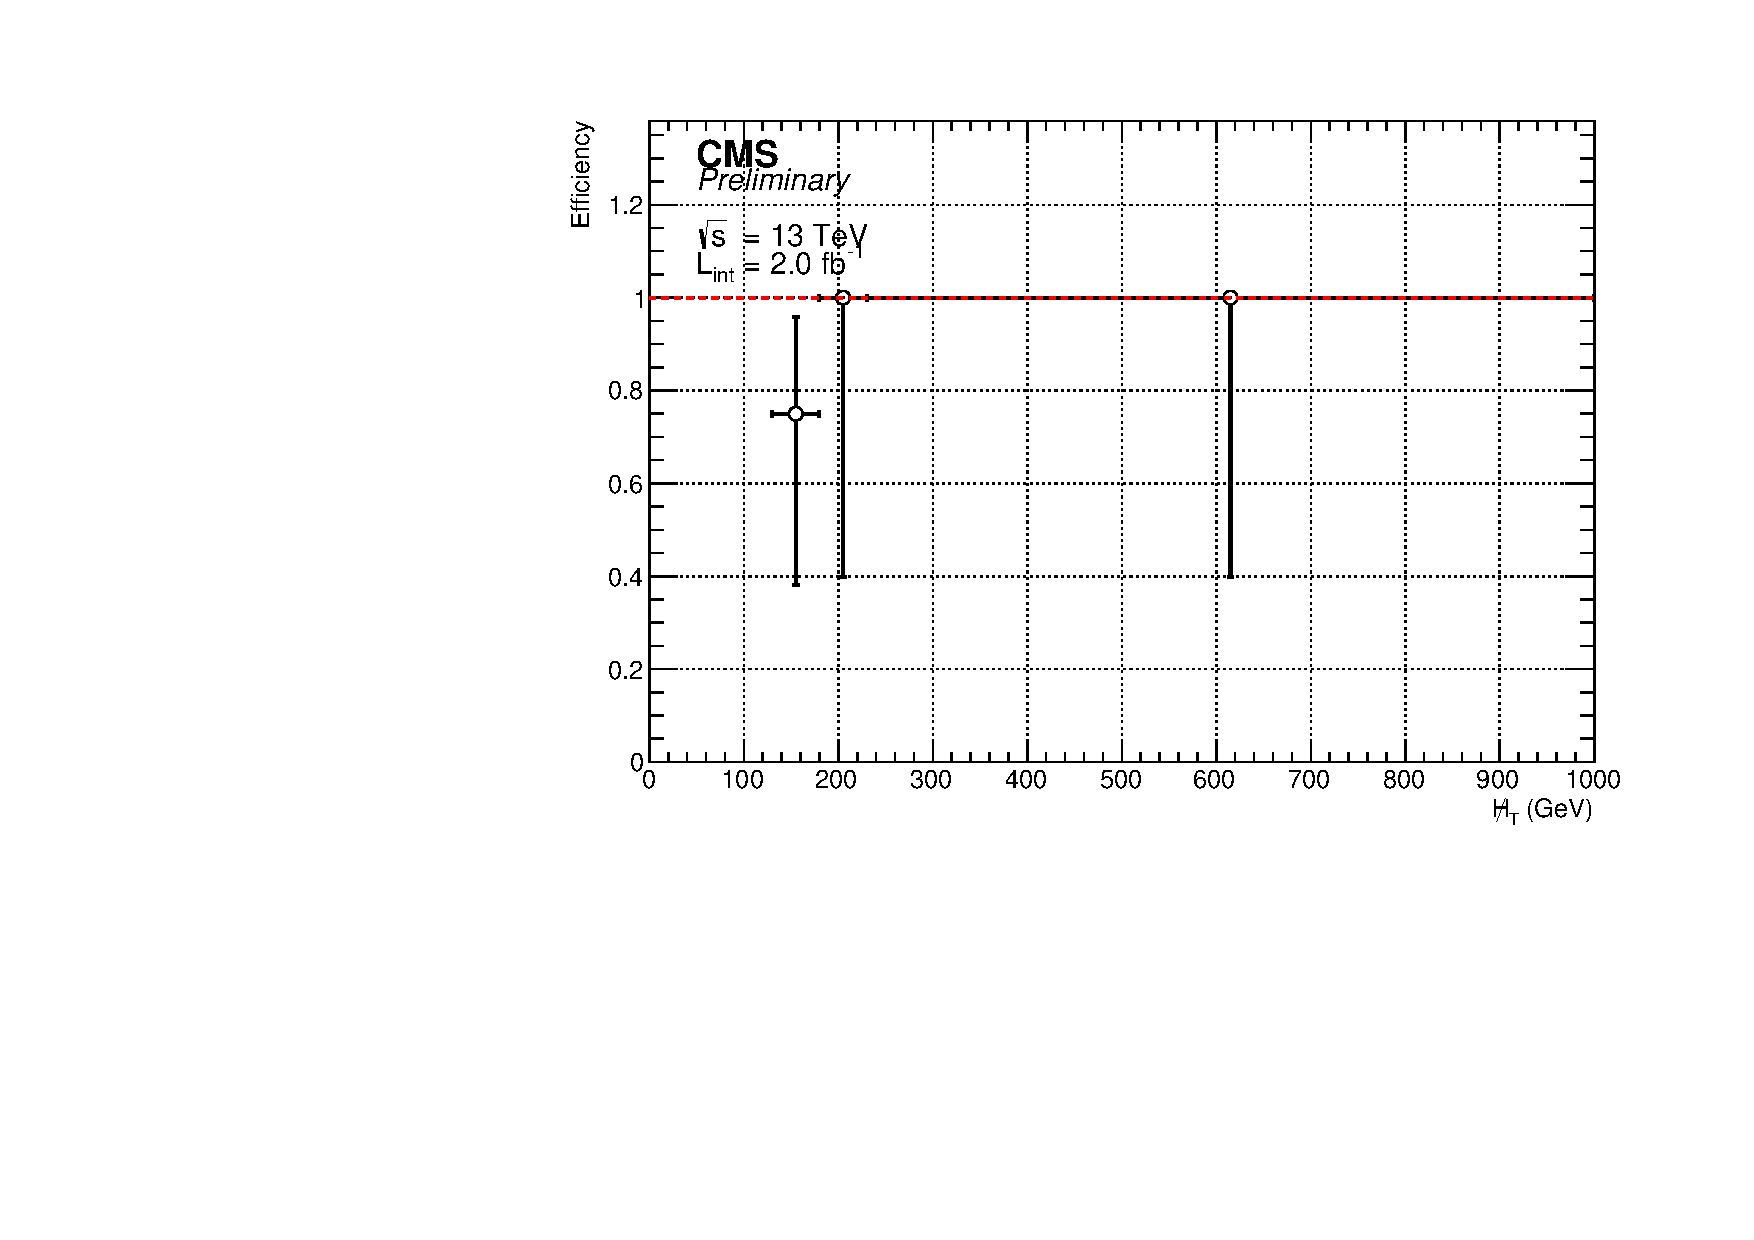
\includegraphics[width=0.4\textwidth]{figures/Trigger/NJetBinned/HLT_AlphaTMonoAll_MoM_eq4j_250to300_mht}} \\
    \subfigure[{\tiny $\scalht = 250\mathrm-300$~GeV, $\njet = 2$ asym.}]{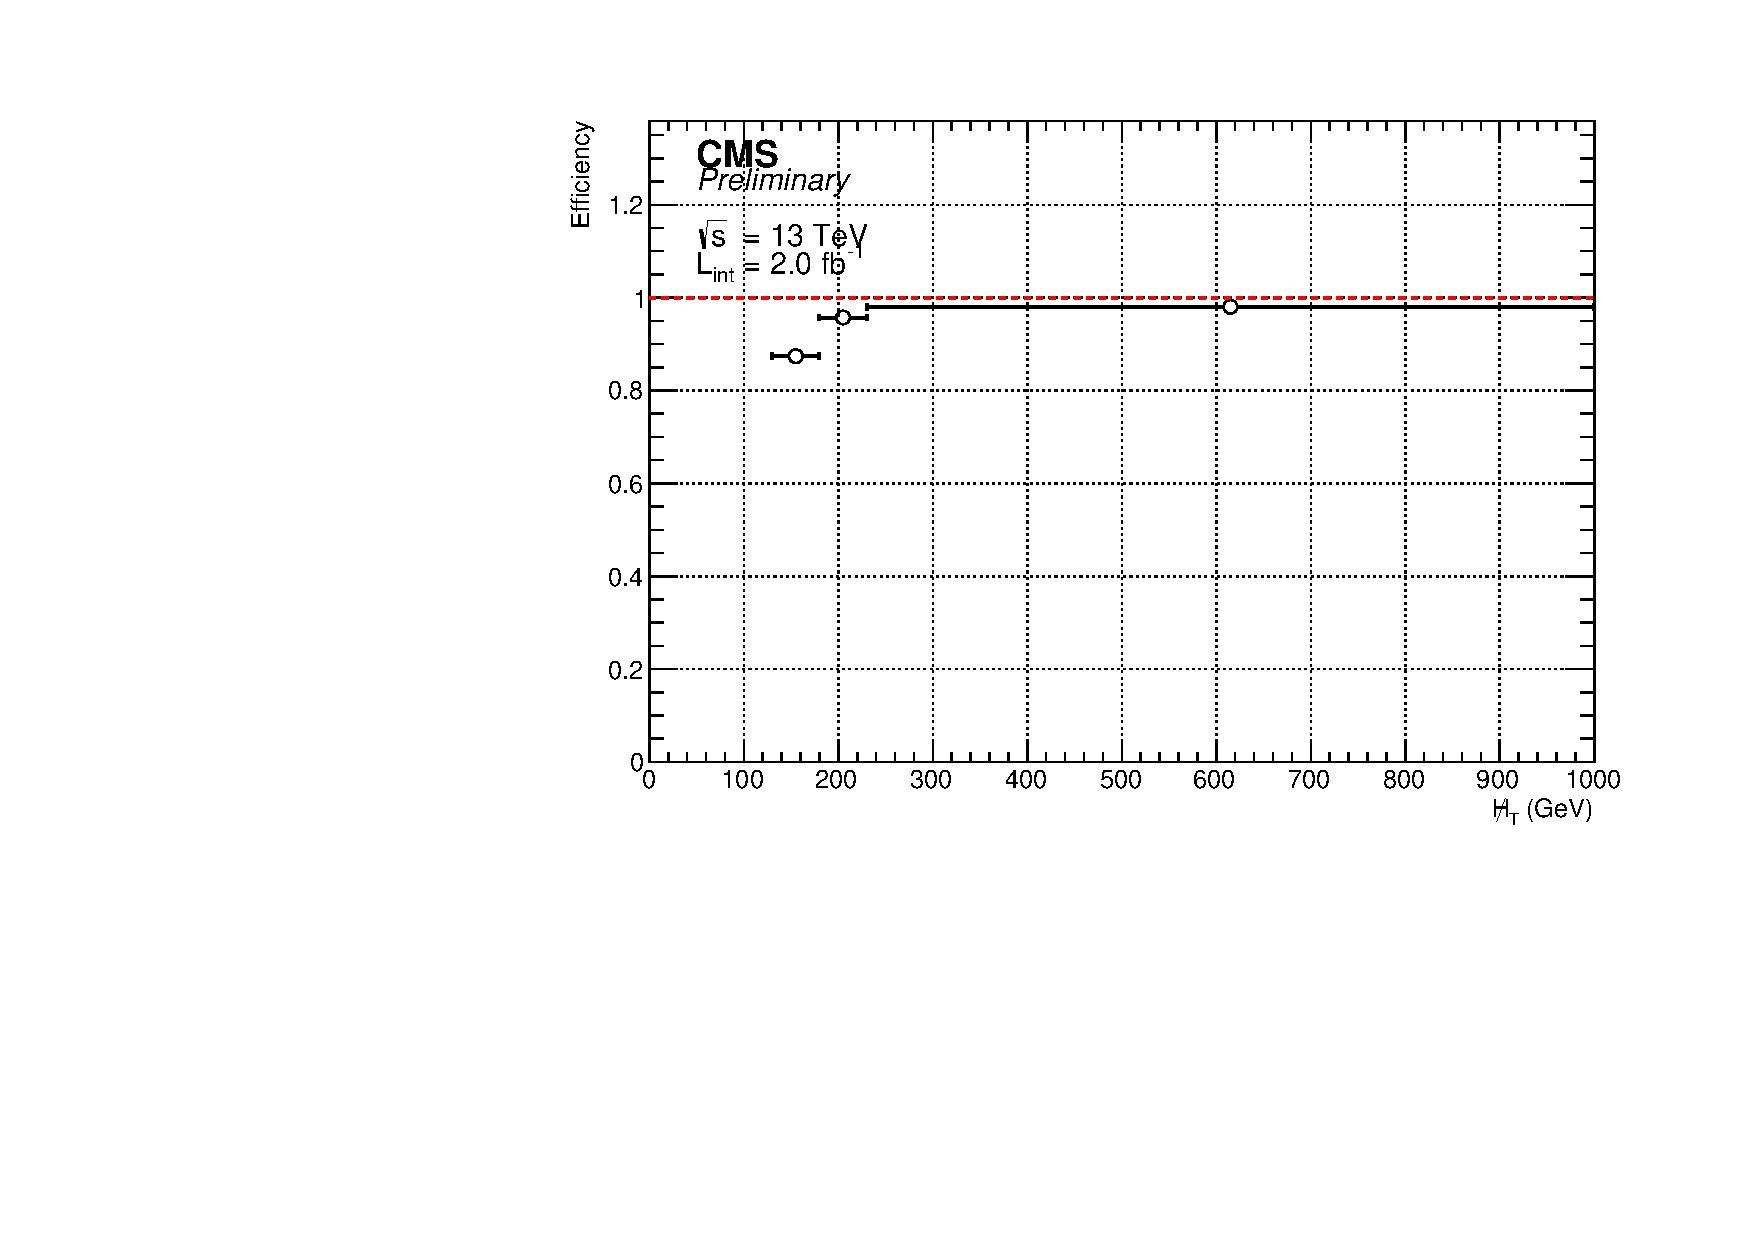
\includegraphics[width=0.4\textwidth]{figures/Trigger/NJetBinned/HLT_AlphaTMonoAll_MoM_eq2a_250to300_mht}}
    \subfigure[{\tiny $\scalht = 250\mathrm-300$~GeV, $\njet = 3$ asym.}]{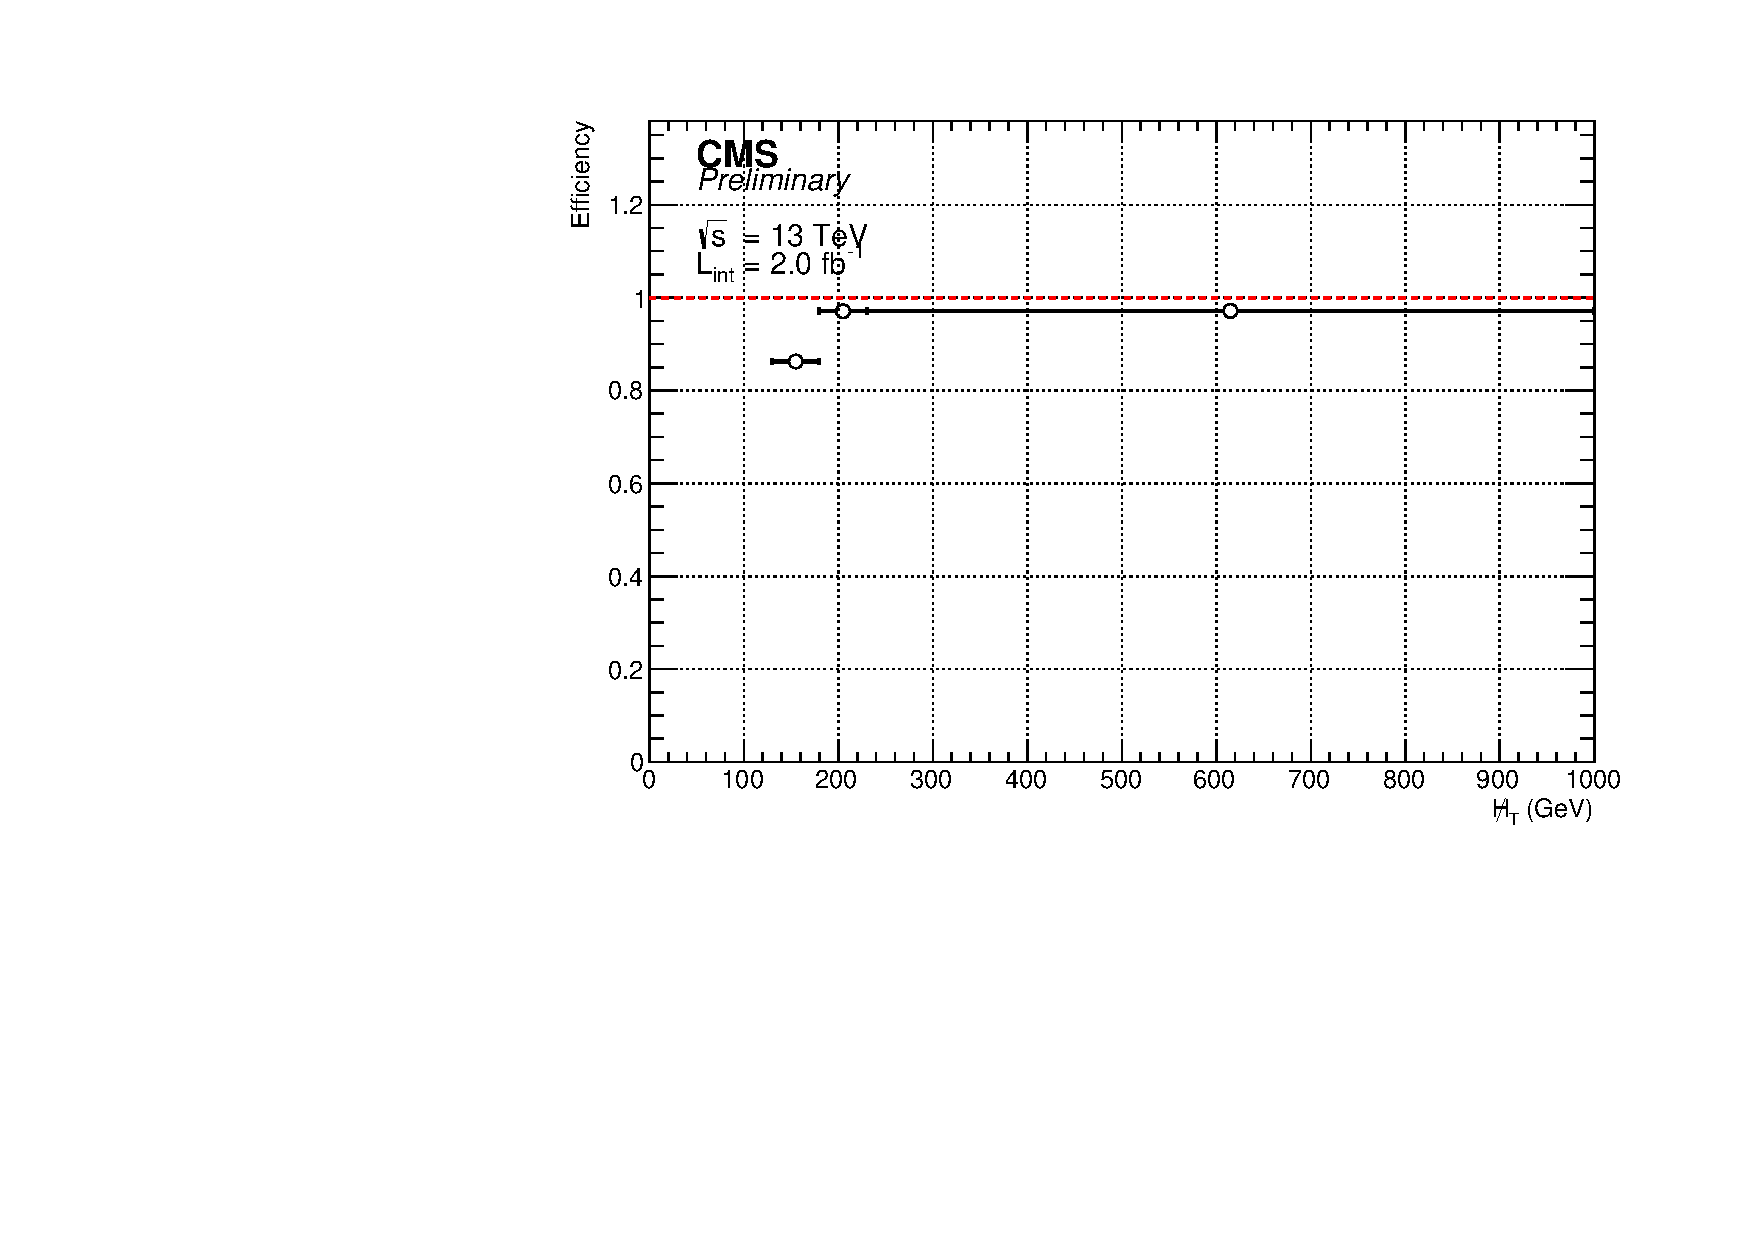
\includegraphics[width=0.4\textwidth]{figures/Trigger/NJetBinned/HLT_AlphaTMonoAll_MoM_eq3a_250to300_mht}} \\
    \subfigure[{\tiny $\scalht = 250\mathrm-300$~GeV, $\njet = 4$ asym.}]{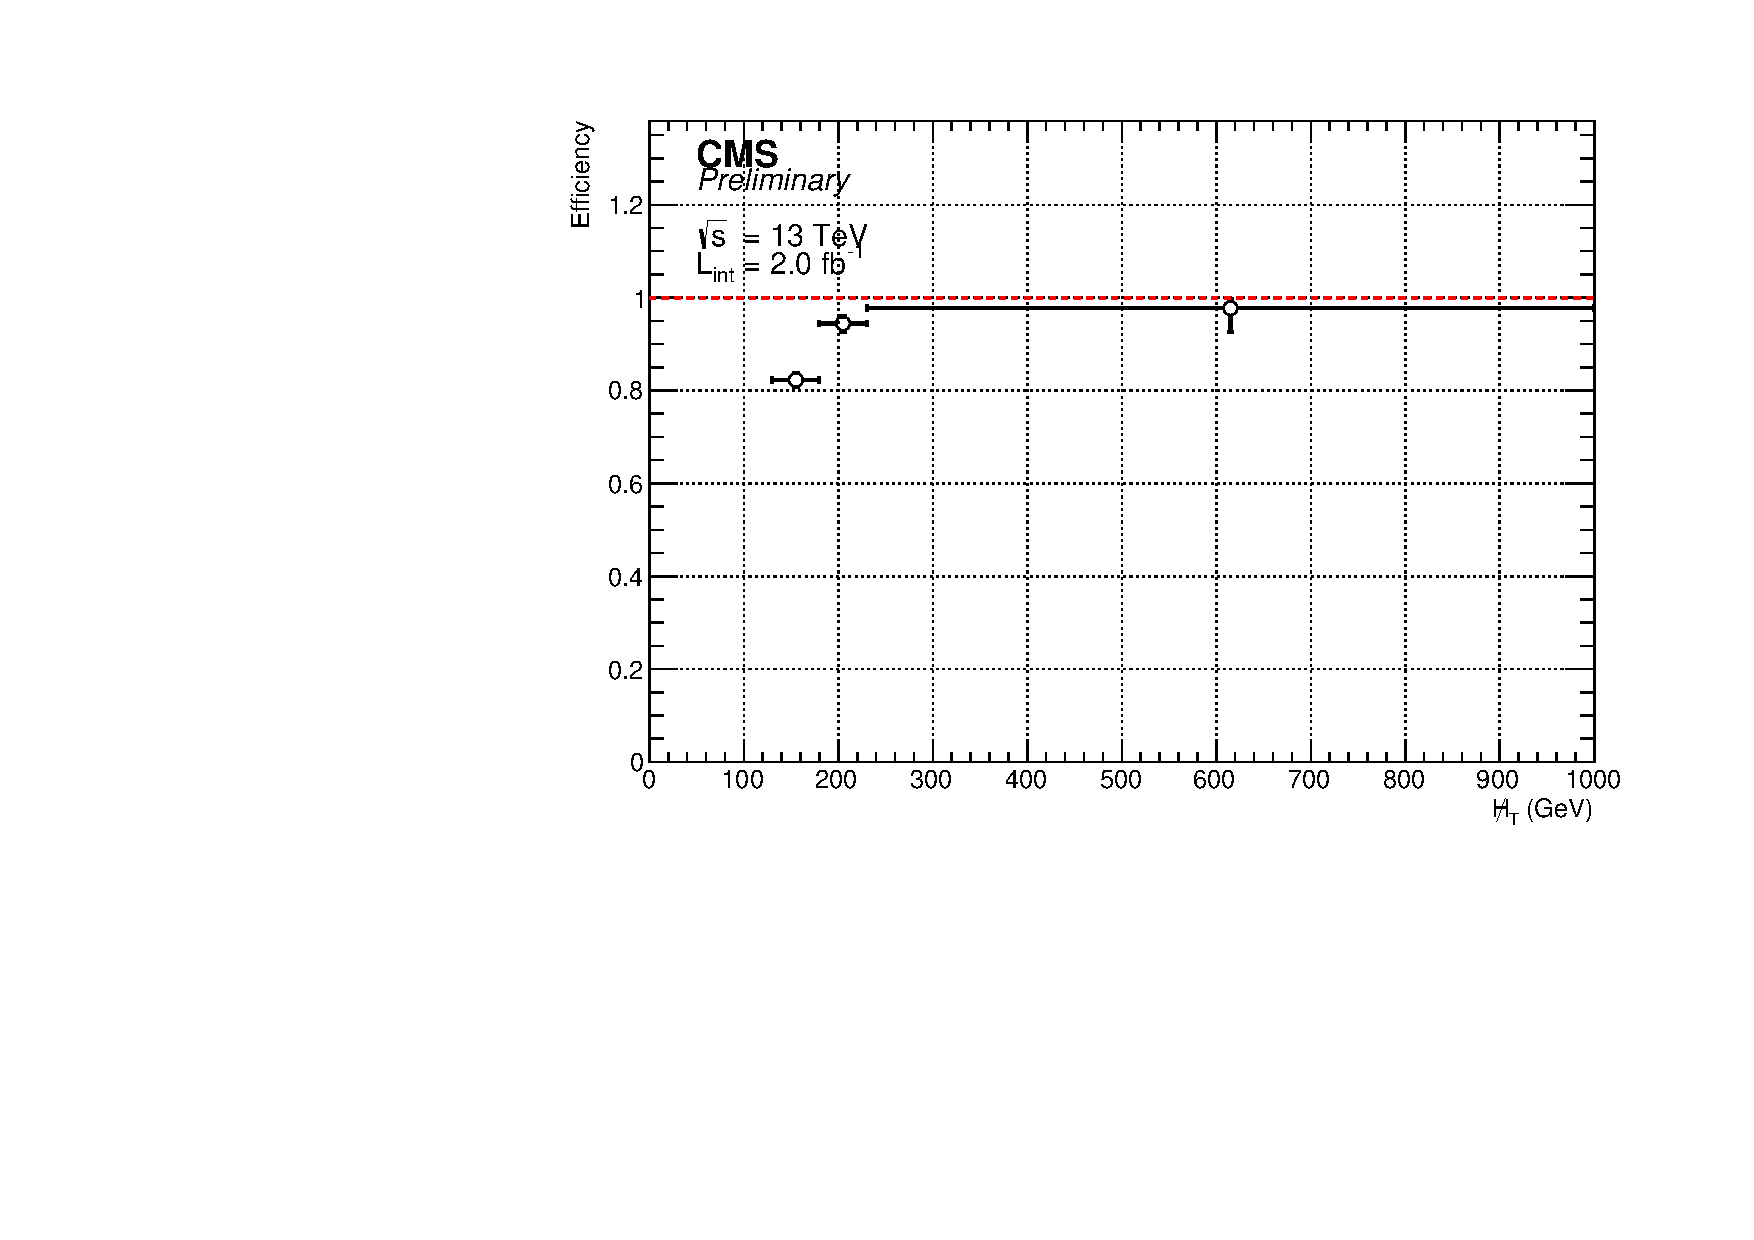
\includegraphics[width=0.4\textwidth]{figures/Trigger/NJetBinned/HLT_AlphaTMonoAll_MoM_eq4a_250to300_mht}}
    \caption{\mht trigger turn-ons in the low \scalht signal region in bins of \njet.}
    \label{fig:turnons_njetbinned}
  \end{center}
\end{figure}

